%%%%%%%%%%%%%%%%%%%%%%%%%%%%%%%%%%%%%%%%%%%%%%%%%
%%%%%%%%%%%%%%%%%%%%%%%%%%%%%%%%%%%%%%%%%%%%%%%%%
\chapter{Results}
\label{chap:results}

In order to evaluate the the algorithms, analysis is organised around three major characteristics of swarm robotics algorithms, namely flexibility, robustness and scalability. Section~\ref{overview} focuses on providing a general overview of algorithm performances, while flexibility of the algorithms over different environmental types and configurations is analysed in Section~\ref{results:flexibility}. The robustness to environmental changes is analysed in Section~\ref{results:robustness} while Section~\ref{results:scability} does a limited exploration of scalability. Section~\ref{results:summary} summarizes the findings of the experimentation. 

\section{General Overview}
\label{overview}

\begin{table}
\centering
    \caption{Overall pairwise one-tailed Mann Whitney U wins and losses, averages and standard deviations for $\sigma$ for each algorithm}
        \label{summarytable}
    \begin{tabular}{l|llll}
    \hline \hline
    Algorithms & Wins & Losses & Average & Std Dev \\ \hline
    Naive      & 1168    & 59042 & 0.528   & 0.394  \\
    Desert Ant  & 42120 & 14557 & 0.643   & 0.387  \\
    Honey Bee   & 45490 & 15179 & 0.807   & 0.294  \\
    \hline
    \end{tabular}
\end{table}

The desert ant, honey-bee and na\"ive foraging algorithms are compared for various robot configurations over various environments. In order to compare two experiments, two one-tailed Wilcoxin tests are performed where the first test determines if the samples in algorithm A are greater than the samples in algorithm B - which is counted as a win and the second test determines if the samples in algorithm A are less than the samples in algorithm B - which is counted as a loss. In order to get an idea of an algorithms performance against the other algorithms, the wins and losses per experiment are counted per algorithm. This statistical analysis approach has been used in \cite{helbig2013performance}. Table \ref{summarytable} shows the sum of the wins and losses per algorithm.

The pairwise Wilcoxon tests indicate that there exists a significant difference between the results of all three foraging algorithms. Desert ant foraging performed better than na\"ive foraging showing the positive effect of site fidelity. The honey bee algorithm out-performed the na\"ive foraging algorithm and desert ant algorithm indicating the positive effect of communication and adaptivity of the honey bee foraging algorithm. The standard deviation is high for all algorithms due to the extremely large variations in the environments provided.

However, these are results for all algorithms over all configurations of robot specialization and thus comparison is premature. In order to perform a real comparison between algorithms, the robot specialization parameter $\tau$ should be optimized in the potential event that there exists an initial configuration for $\tau$ that performs best across all environment types and robot configurations addressed in the analysis. This study rather focuses on a sensitivity study of the algorithms to a variety of environmental, and algorithmic parameters.


\section{Flexibility}
\label{results:flexibility}

In real life environments, it's rarely feasible to optimize parameters per the environment where a swarm of robots needs to be introduced. As a result, it's important that swarm robotics algorithms are insensitive to types of environment and either have a set of parameters that generalize well or have the ability to adapt their parameters to an unseen environment.

In order to determine the flexibility of the three proposed foraging algorithms, the effect of the ratio of item types in the environment and the effect on different types of distributions of prioritized and non-prioritized items in the environments is analysed. The more insensitive an algorithm is to the change in environmental parameters, the more flexible the algorithm can be considered to be. 

\subsection{Environment Item Ratio}
\label{results:ratio}

\begin{table} [h]
    \caption{Effect of environment ratio $r$ on prioritized item foraging per algorithm}
    \label{generalratio}
	\centering
	\footnotesize
	\begin{tabular} {|l|l|l|l|}
		\hline
		Environment Ratio & Na\"ive & Desert Ant & Honey Bee \\
		\hline
		0 & 1 (0)  & 1 (0)  & 1 (0)  \\
		0.2 & 0.339535 (0.376654)  & 0.445135 (0.407285)  & 0.487141 (0.39498)  \\
		0.25 & 0.334883 (0.373433)  & 0.439328 (0.404576)  & 0.477255 (0.393016)  \\
		0.333333 & 0.333027 (0.366004)  & 0.440543 (0.39699)  & 0.478846 (0.384682)  \\
		0.5 & 0.322906 (0.353746)  & 0.433707 (0.386719)  & 0.472925 (0.375211)  \\
		0.666667 & 0.317141 (0.346356)  & 0.428729 (0.380685)  & 0.475938 (0.370087)  \\
		0.75 & 0.313083 (0.342088)  & 0.425262 (0.377452)  & 0.478247 (0.366827)  \\
		0.8 & 0.310814 (0.340525)  & 0.424046 (0.376479)  & 0.480269 (0.365919)  \\
		1 & 0.302589 (0.3297)  & 0.411166 (0.369788)  & 0.493483 (0.360374)  \\
		\hline
	\end{tabular}
\end{table}

Environment item ratio refers to the ratio of prioritized items to non-prioritized items $r$ in the foraging environment. In order to truly analyse the effects of the environment, one should optimize each algorithm for all the environments since there may exist a parameter set for the algorithms that performs well over all environments. For this reason, we first analyse two hypotheses related to the dependency of the performance of an algorithm in environments with a particular item ratio and the ratio of specialization of the robots themselves.

\begin{figure}[!htb]
\centering
\resizebox{\textwidth}{!}{% GNUPLOT: LaTeX picture with Postscript
\begingroup
  \makeatletter
  \providecommand\color[2][]{%
    \GenericError{(gnuplot) \space\space\space\@spaces}{%
      Package color not loaded in conjunction with
      terminal option `colourtext'%
    }{See the gnuplot documentation for explanation.%
    }{Either use 'blacktext' in gnuplot or load the package
      color.sty in LaTeX.}%
    \renewcommand\color[2][]{}%
  }%
  \providecommand\includegraphics[2][]{%
    \GenericError{(gnuplot) \space\space\space\@spaces}{%
      Package graphicx or graphics not loaded%
    }{See the gnuplot documentation for explanation.%
    }{The gnuplot epslatex terminal needs graphicx.sty or graphics.sty.}%
    \renewcommand\includegraphics[2][]{}%
  }%
  \providecommand\rotatebox[2]{#2}%
  \@ifundefined{ifGPcolor}{%
    \newif\ifGPcolor
    \GPcolorfalse
  }{}%
  \@ifundefined{ifGPblacktext}{%
    \newif\ifGPblacktext
    \GPblacktexttrue
  }{}%
  % define a \g@addto@macro without @ in the name:
  \let\gplgaddtomacro\g@addto@macro
  % define empty templates for all commands taking text:
  \gdef\gplbacktext{}%
  \gdef\gplfronttext{}%
  \makeatother
  \ifGPblacktext
    % no textcolor at all
    \def\colorrgb#1{}%
    \def\colorgray#1{}%
  \else
    % gray or color?
    \ifGPcolor
      \def\colorrgb#1{\color[rgb]{#1}}%
      \def\colorgray#1{\color[gray]{#1}}%
      \expandafter\def\csname LTw\endcsname{\color{white}}%
      \expandafter\def\csname LTb\endcsname{\color{black}}%
      \expandafter\def\csname LTa\endcsname{\color{black}}%
      \expandafter\def\csname LT0\endcsname{\color[rgb]{1,0,0}}%
      \expandafter\def\csname LT1\endcsname{\color[rgb]{0,1,0}}%
      \expandafter\def\csname LT2\endcsname{\color[rgb]{0,0,1}}%
      \expandafter\def\csname LT3\endcsname{\color[rgb]{1,0,1}}%
      \expandafter\def\csname LT4\endcsname{\color[rgb]{0,1,1}}%
      \expandafter\def\csname LT5\endcsname{\color[rgb]{1,1,0}}%
      \expandafter\def\csname LT6\endcsname{\color[rgb]{0,0,0}}%
      \expandafter\def\csname LT7\endcsname{\color[rgb]{1,0.3,0}}%
      \expandafter\def\csname LT8\endcsname{\color[rgb]{0.5,0.5,0.5}}%
    \else
      % gray
      \def\colorrgb#1{\color{black}}%
      \def\colorgray#1{\color[gray]{#1}}%
      \expandafter\def\csname LTw\endcsname{\color{white}}%
      \expandafter\def\csname LTb\endcsname{\color{black}}%
      \expandafter\def\csname LTa\endcsname{\color{black}}%
      \expandafter\def\csname LT0\endcsname{\color{black}}%
      \expandafter\def\csname LT1\endcsname{\color{black}}%
      \expandafter\def\csname LT2\endcsname{\color{black}}%
      \expandafter\def\csname LT3\endcsname{\color{black}}%
      \expandafter\def\csname LT4\endcsname{\color{black}}%
      \expandafter\def\csname LT5\endcsname{\color{black}}%
      \expandafter\def\csname LT6\endcsname{\color{black}}%
      \expandafter\def\csname LT7\endcsname{\color{black}}%
      \expandafter\def\csname LT8\endcsname{\color{black}}%
    \fi
  \fi
  \setlength{\unitlength}{0.0500bp}%
  \begin{picture}(7200.00,5040.00)%
    \gplgaddtomacro\gplbacktext{%
      \csname LTb\endcsname%
      \put(946,704){\makebox(0,0)[r]{\strut{} 0.3}}%
      \put(946,1229){\makebox(0,0)[r]{\strut{} 0.4}}%
      \put(946,1754){\makebox(0,0)[r]{\strut{} 0.5}}%
      \put(946,2279){\makebox(0,0)[r]{\strut{} 0.6}}%
      \put(946,2804){\makebox(0,0)[r]{\strut{} 0.7}}%
      \put(946,3329){\makebox(0,0)[r]{\strut{} 0.8}}%
      \put(946,3854){\makebox(0,0)[r]{\strut{} 0.9}}%
      \put(946,4379){\makebox(0,0)[r]{\strut{} 1}}%
      \put(1078,484){\makebox(0,0){\strut{} 0}}%
      \put(2223,484){\makebox(0,0){\strut{} 0.2}}%
      \put(3368,484){\makebox(0,0){\strut{} 0.4}}%
      \put(4513,484){\makebox(0,0){\strut{} 0.6}}%
      \put(5658,484){\makebox(0,0){\strut{} 0.8}}%
      \put(6803,484){\makebox(0,0){\strut{} 1}}%
      \put(176,2541){\rotatebox{-270}{\makebox(0,0){\strut{}Prioritized items over time ($\sigma$)}}}%
      \put(3940,154){\makebox(0,0){\strut{}Item Type Ratio ($r$)}}%
      \put(3940,4709){\makebox(0,0){\strut{}Prioritized items over time for each algorithm for item type ratios}}%
    }%
    \gplgaddtomacro\gplfronttext{%
      \csname LTb\endcsname%
      \put(5816,4206){\makebox(0,0)[r]{\strut{}Na\"ive}}%
      \csname LTb\endcsname%
      \put(5816,3986){\makebox(0,0)[r]{\strut{}Desert Ant}}%
      \csname LTb\endcsname%
      \put(5816,3766){\makebox(0,0)[r]{\strut{}Honey Bee}}%
    }%
    \gplbacktext
    \put(0,0){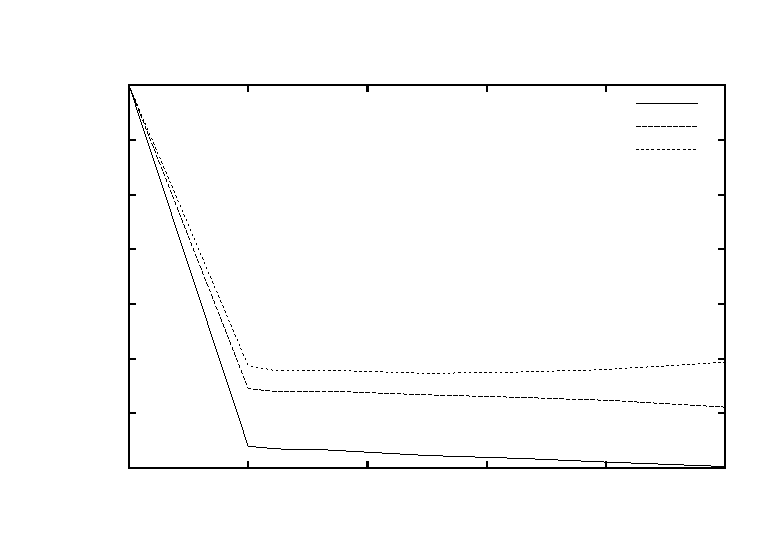
\includegraphics{chapters/chapter6/graphs/gold_ratio}}%
    \gplfronttext
  \end{picture}%
\endgroup
}
\caption{Prioritized items over time over environment ratio $r$ for each algorithm }
\label{ratiogoldplot}
\end{figure}


\begin{figure}[!htb]
\centering
\resizebox{\textwidth}{!}{% GNUPLOT: LaTeX picture with Postscript
\begingroup
  \makeatletter
  \providecommand\color[2][]{%
    \GenericError{(gnuplot) \space\space\space\@spaces}{%
      Package color not loaded in conjunction with
      terminal option `colourtext'%
    }{See the gnuplot documentation for explanation.%
    }{Either use 'blacktext' in gnuplot or load the package
      color.sty in LaTeX.}%
    \renewcommand\color[2][]{}%
  }%
  \providecommand\includegraphics[2][]{%
    \GenericError{(gnuplot) \space\space\space\@spaces}{%
      Package graphicx or graphics not loaded%
    }{See the gnuplot documentation for explanation.%
    }{The gnuplot epslatex terminal needs graphicx.sty or graphics.sty.}%
    \renewcommand\includegraphics[2][]{}%
  }%
  \providecommand\rotatebox[2]{#2}%
  \@ifundefined{ifGPcolor}{%
    \newif\ifGPcolor
    \GPcolorfalse
  }{}%
  \@ifundefined{ifGPblacktext}{%
    \newif\ifGPblacktext
    \GPblacktexttrue
  }{}%
  % define a \g@addto@macro without @ in the name:
  \let\gplgaddtomacro\g@addto@macro
  % define empty templates for all commands taking text:
  \gdef\gplbacktext{}%
  \gdef\gplfronttext{}%
  \makeatother
  \ifGPblacktext
    % no textcolor at all
    \def\colorrgb#1{}%
    \def\colorgray#1{}%
  \else
    % gray or color?
    \ifGPcolor
      \def\colorrgb#1{\color[rgb]{#1}}%
      \def\colorgray#1{\color[gray]{#1}}%
      \expandafter\def\csname LTw\endcsname{\color{white}}%
      \expandafter\def\csname LTb\endcsname{\color{black}}%
      \expandafter\def\csname LTa\endcsname{\color{black}}%
      \expandafter\def\csname LT0\endcsname{\color[rgb]{1,0,0}}%
      \expandafter\def\csname LT1\endcsname{\color[rgb]{0,1,0}}%
      \expandafter\def\csname LT2\endcsname{\color[rgb]{0,0,1}}%
      \expandafter\def\csname LT3\endcsname{\color[rgb]{1,0,1}}%
      \expandafter\def\csname LT4\endcsname{\color[rgb]{0,1,1}}%
      \expandafter\def\csname LT5\endcsname{\color[rgb]{1,1,0}}%
      \expandafter\def\csname LT6\endcsname{\color[rgb]{0,0,0}}%
      \expandafter\def\csname LT7\endcsname{\color[rgb]{1,0.3,0}}%
      \expandafter\def\csname LT8\endcsname{\color[rgb]{0.5,0.5,0.5}}%
    \else
      % gray
      \def\colorrgb#1{\color{black}}%
      \def\colorgray#1{\color[gray]{#1}}%
      \expandafter\def\csname LTw\endcsname{\color{white}}%
      \expandafter\def\csname LTb\endcsname{\color{black}}%
      \expandafter\def\csname LTa\endcsname{\color{black}}%
      \expandafter\def\csname LT0\endcsname{\color{black}}%
      \expandafter\def\csname LT1\endcsname{\color{black}}%
      \expandafter\def\csname LT2\endcsname{\color{black}}%
      \expandafter\def\csname LT3\endcsname{\color{black}}%
      \expandafter\def\csname LT4\endcsname{\color{black}}%
      \expandafter\def\csname LT5\endcsname{\color{black}}%
      \expandafter\def\csname LT6\endcsname{\color{black}}%
      \expandafter\def\csname LT7\endcsname{\color{black}}%
      \expandafter\def\csname LT8\endcsname{\color{black}}%
    \fi
  \fi
  \setlength{\unitlength}{0.0500bp}%
  \begin{picture}(7200.00,5040.00)%
    \gplgaddtomacro\gplbacktext{%
      \csname LTb\endcsname%
      \put(946,704){\makebox(0,0)[r]{\strut{} 0.3}}%
      \put(946,1229){\makebox(0,0)[r]{\strut{} 0.4}}%
      \put(946,1754){\makebox(0,0)[r]{\strut{} 0.5}}%
      \put(946,2279){\makebox(0,0)[r]{\strut{} 0.6}}%
      \put(946,2804){\makebox(0,0)[r]{\strut{} 0.7}}%
      \put(946,3329){\makebox(0,0)[r]{\strut{} 0.8}}%
      \put(946,3854){\makebox(0,0)[r]{\strut{} 0.9}}%
      \put(946,4379){\makebox(0,0)[r]{\strut{} 1}}%
      \put(1078,484){\makebox(0,0){\strut{} 0}}%
      \put(2223,484){\makebox(0,0){\strut{} 0.2}}%
      \put(3368,484){\makebox(0,0){\strut{} 0.4}}%
      \put(4513,484){\makebox(0,0){\strut{} 0.6}}%
      \put(5658,484){\makebox(0,0){\strut{} 0.8}}%
      \put(6803,484){\makebox(0,0){\strut{} 1}}%
      \put(176,2541){\rotatebox{-270}{\makebox(0,0){\strut{}Non-prioritized items over time ($\sigma$)}}}%
      \put(3940,154){\makebox(0,0){\strut{}Item Type Ratio ($r$)}}%
      \put(3940,4709){\makebox(0,0){\strut{}Non-prioritized items over time for each algorithm for item type ratios}}%
    }%
    \gplgaddtomacro\gplfronttext{%
      \csname LTb\endcsname%
      \put(5816,4206){\makebox(0,0)[r]{\strut{}Na\"ive}}%
      \csname LTb\endcsname%
      \put(5816,3986){\makebox(0,0)[r]{\strut{}Desert Ant}}%
      \csname LTb\endcsname%
      \put(5816,3766){\makebox(0,0)[r]{\strut{}Honey Bee}}%
    }%
    \gplbacktext
    \put(0,0){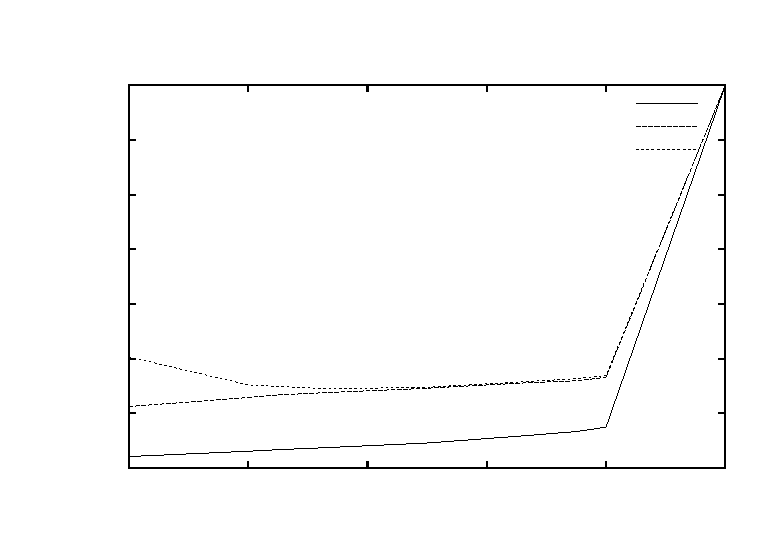
\includegraphics{chapters/chapter6/graphs/waste_ratio}}%
    \gplfronttext
  \end{picture}%
\endgroup
}
\caption{Non-prioritized items over time over environment ratio $r$ for each algorithm}
\label{ratiowasteplot}
\end{figure}

\subsubsection{The Relationship between Environment Item Ratio and Specialization Ratio of Robots}
\label{relationship}

The next section addresses the following hypotheses:
\begin{enumerate}
\item An algorithm that forages a portion of non-prioritized items will have greater performance than an algorithm that does not forage any non-prioritized items.
\item Algorithm performance depends on the environment ratio $r$ and the specialization ratio $\tau$. As $r$ increases, the value of $\tau$ that yields the greatest value of $\sigma$, $\tau_{best}$, will increase approximately linearly for the na\"ive and desert ant algorithms, while the performance of the honey bee algorithm will be independent of $r$ due to division of labour.
\end{enumerate}

An algorithm configured with $\tau=1$ indicates that only prioritized items are foraged. By analysing Table \ref{ratio}, for the na\"ive and desert ant algorithms, for all values of $r$ where $r \neq 1$, $\tau_{best}$ is never equal to $1$, thus the hypothesis that the algorithms achieved the best performance when some robots are configured to forage non-prioritized items is true. The result is likely because non-prioritized items are moved out of the way to allow for easier, faster access to prioritized items or allow access to inaccessible prioritized items.


\begin{table} [h]
     \caption{The performance, $\sigma$, for each foraging algorithm, for each combinations of $r$ and $\tau$. If $\tau_{best}$ exists, $\tau_{best}$ is provided. The best value of $\sigma$ is shown in bold.}
     \label{ratio}
	\centering
	\footnotesize
    \begin{tabular}{|c|c||l|l|l|l|l|l|l|l|l||l|}
	\hline    & & \multicolumn{9}{ |c|| } {$\tau$} &   \\ 
    \cline{3-11}
\multirow{-2}{*}{Algorithm}  &  \multirow{-2}{*}{$r$} & 0     & 0.2   & 0.25  & 0.333 & 0.5   & 0.667  & 0.75  & 0.8    & 1   & \multirow{-2}{*}{$\tau_{best}$ } \\ \hline
    &0     & 1 & 1     & 1     & 1     & 1     & 1     & 1     & 1     & 1     & \\
    &0.2   & 0 & 0.492 & 0.526 & 0.567 & \textbf{0.597} & 0.595 & 0.587 & 0.577 & 0.471 & 0.5 \\
    &0.25  & 0 & 0.484 & 0.526 & 0.557 & 0.588 & \textbf{0.595} & 0.585 & 0.575 & 0.477 & 0.667\\
    &0.333 & 0 & 0.467 & 0.507 & 0.544 & 0.586 & \textbf{0.596} & 0.592 & 0.584 & 0.495 & 0.667\\
    &0.5   & 0 & 0.428 & 0.46  & 0.508 & 0.568 & 0.588 & \textbf{0.591} & 0.589 & 0.528 & 0.75\\
    &0.667 & 0 & 0.4   & 0.433 & 0.487 & 0.544 & 0.583 & \textbf{0.591} & 0.593 & 0.554 & 0.75 \\
    &0.75  & 0 & 0.377 & 0.425 & 0.47  & 0.531 & 0.576 & 0.585 & \textbf{0.591} & 0.567 & 0.8\\
    &0.8   & 0 & 0.372 & 0.409 & 0.455 & 0.53  & 0.571 & 0.584 & \textbf{0.592} & 0.575 & 0.8\\
\multirow{-9}{*}{Na\"ive}&    1     & 0 & 0.336 & 0.375 & 0.433 & 0.5   & 0.552 & 0.57  & 0.581 & \textbf{0.618} & 1\\
     \hline
 &   0                    & 1 & 1     & 1     & 1     & 1     & 1     & 1     & 1     & 1       &    \\
&    0.2                  & 0 & 0.698 & 0.724 & \textbf{0.737} & \textbf{0.737} & 0.712 & 0.694 & 0.67  & 0.519 & 0.333\\
&    0.25                 & 0 & 0.678 & 0.711 & 0.73  & \textbf{0.735} & 0.715 & 0.697 & 0.673 & 0.530 & 0.5 \\
&    0.333                & 0 & 0.65  & 0.693 & 0.722 & \textbf{0.739} & 0.725 & 0.71  & 0.686 & 0.562 & 0.5\\
&    0.5                  & 0 & 0.596 & 0.645 & 0.684 & 0.729 & \textbf{0.734} & 0.725 & 0.701 & 0.621 & 0.667\\
&    0.667                & 0 & 0.554 & 0.607 & 0.648 & 0.706 & 0.737 & \textbf{0.738} & 0.716 & 0.675 & 0.75\\
&    0.75                 & 0 & 0.533 & 0.587 & 0.63  & 0.691 & 0.731 & \textbf{0.739} & 0.72  & 0.703  & 0.75 \\
&    0.8                  & 0 & 0.523 & 0.577 & 0.62  & 0.682 & 0.725 & 0.736 & \textbf{0.74}  & 0.718 & 0.8\\
\multirow{-9}{*}{Desert Ant}&    1                    & 0 & 0.488 & 0.543 & 0.588 & 0.654 & 0.702 & 0.718 & 0.726 & \textbf{0.758} & 1\\ \hline
    %Honey Bee
&        0  & 1     & 1     & 1     & 1     & 1     & 1     & 1     & 1     & 1  &   \\
&    0.2                  & \textbf{0.687} &\textbf{0.687} & 0.686 & 0.686 & 0.686 & 0.685 & 0.686 & 0.685 & \textbf{0.687} &\\
&    0.25                 & 0.678 & \textbf{0.679} & 0.678 & 0.678 &\textbf{0.679} & \textbf{0.679} & 0.678 & 0.677 & \textbf{0.679} &\\
&    0.333                & \textbf{0.674} & \textbf{0.674} & \textbf{0.674} & \textbf{0.674} & \textbf{0.674} & \textbf{0.674} & 0.673 & \textbf{0.674} &\textbf{0.674} &\\
&    0.5                  & 0.668 & \textbf{0.669} & 0.668 & 0.668 & 0.668 & 0.668 & 0.668 & 0.668 & \textbf{0.669} &\\
&    0.667                & 0.671 & 0.671 & 0.671 & 0.671 & 0.671 & \textbf{0.672} & 0.671 & 0.671 & 0.671 &\\
&    0.75                 & 0.672 & \textbf{0.673} & 0.671 & 0.671 & 0.672 &\textbf{0.673} & 0.672 & \textbf{0.673} & \textbf{0.673}&\\
&    0.8                  & 0.674 & 0.674 & 0.674 & 0.674 & 0.674 & \textbf{0.675} &  \textbf{0.675} &  \textbf{0.675} & \textbf{0.675}& \\
\multirow{-9}{*}{Honey Bee}&    1                    & \textbf{0.691} & 0.69  & \textbf{0.691} & 0.69  & \textbf{0.691} &  \textbf{0.691}& 0.69  & 0.69  & 0.69  &\\ \hline

    \end{tabular}

\end{table}

Fig \ref{desertantplot} shows the region in parameter space where the desert ant algorithm performs the best. The na\"ive and desert ant algorithms performed best when $\tau$ was slightly greater than $r$. The existence of the relationship motivates the development of an algorithm that adapts $\tau$ to correspond the environment item ratio $r$.

\begin{figure}[!htb]
\centering
\resizebox{0.8\textwidth}{!}{% GNUPLOT: LaTeX picture with Postscript
\begingroup
  \makeatletter
  \providecommand\color[2][]{%
    \GenericError{(gnuplot) \space\space\space\@spaces}{%
      Package color not loaded in conjunction with
      terminal option `colourtext'%
    }{See the gnuplot documentation for explanation.%
    }{Either use 'blacktext' in gnuplot or load the package
      color.sty in LaTeX.}%
    \renewcommand\color[2][]{}%
  }%
  \providecommand\includegraphics[2][]{%
    \GenericError{(gnuplot) \space\space\space\@spaces}{%
      Package graphicx or graphics not loaded%
    }{See the gnuplot documentation for explanation.%
    }{The gnuplot epslatex terminal needs graphicx.sty or graphics.sty.}%
    \renewcommand\includegraphics[2][]{}%
  }%
  \providecommand\rotatebox[2]{#2}%
  \@ifundefined{ifGPcolor}{%
    \newif\ifGPcolor
    \GPcolorfalse
  }{}%
  \@ifundefined{ifGPblacktext}{%
    \newif\ifGPblacktext
    \GPblacktexttrue
  }{}%
  % define a \g@addto@macro without @ in the name:
  \let\gplgaddtomacro\g@addto@macro
  % define empty templates for all commands taking text:
  \gdef\gplbacktext{}%
  \gdef\gplfronttext{}%
  \makeatother
  \ifGPblacktext
    % no textcolor at all
    \def\colorrgb#1{}%
    \def\colorgray#1{}%
  \else
    % gray or color?
    \ifGPcolor
      \def\colorrgb#1{\color[rgb]{#1}}%
      \def\colorgray#1{\color[gray]{#1}}%
      \expandafter\def\csname LTw\endcsname{\color{white}}%
      \expandafter\def\csname LTb\endcsname{\color{black}}%
      \expandafter\def\csname LTa\endcsname{\color{black}}%
      \expandafter\def\csname LT0\endcsname{\color[rgb]{1,0,0}}%
      \expandafter\def\csname LT1\endcsname{\color[rgb]{0,1,0}}%
      \expandafter\def\csname LT2\endcsname{\color[rgb]{0,0,1}}%
      \expandafter\def\csname LT3\endcsname{\color[rgb]{1,0,1}}%
      \expandafter\def\csname LT4\endcsname{\color[rgb]{0,1,1}}%
      \expandafter\def\csname LT5\endcsname{\color[rgb]{1,1,0}}%
      \expandafter\def\csname LT6\endcsname{\color[rgb]{0,0,0}}%
      \expandafter\def\csname LT7\endcsname{\color[rgb]{1,0.3,0}}%
      \expandafter\def\csname LT8\endcsname{\color[rgb]{0.5,0.5,0.5}}%
    \else
      % gray
      \def\colorrgb#1{\color{black}}%
      \def\colorgray#1{\color[gray]{#1}}%
      \expandafter\def\csname LTw\endcsname{\color{white}}%
      \expandafter\def\csname LTb\endcsname{\color{black}}%
      \expandafter\def\csname LTa\endcsname{\color{black}}%
      \expandafter\def\csname LT0\endcsname{\color{black}}%
      \expandafter\def\csname LT1\endcsname{\color{black}}%
      \expandafter\def\csname LT2\endcsname{\color{black}}%
      \expandafter\def\csname LT3\endcsname{\color{black}}%
      \expandafter\def\csname LT4\endcsname{\color{black}}%
      \expandafter\def\csname LT5\endcsname{\color{black}}%
      \expandafter\def\csname LT6\endcsname{\color{black}}%
      \expandafter\def\csname LT7\endcsname{\color{black}}%
      \expandafter\def\csname LT8\endcsname{\color{black}}%
    \fi
  \fi
  \setlength{\unitlength}{0.0500bp}%
  \begin{picture}(7200.00,5040.00)%
    \gplgaddtomacro\gplbacktext{%
      \csname LTb\endcsname%
      \put(946,704){\makebox(0,0)[r]{\strut{} 0.2}}%
      \put(946,1213){\makebox(0,0)[r]{\strut{} 0.3}}%
      \put(946,1722){\makebox(0,0)[r]{\strut{} 0.4}}%
      \put(946,2231){\makebox(0,0)[r]{\strut{} 0.5}}%
      \put(946,2740){\makebox(0,0)[r]{\strut{} 0.6}}%
      \put(946,3248){\makebox(0,0)[r]{\strut{} 0.7}}%
      \put(946,3757){\makebox(0,0)[r]{\strut{} 0.8}}%
      \put(946,4266){\makebox(0,0)[r]{\strut{} 0.9}}%
      \put(946,4775){\makebox(0,0)[r]{\strut{} 1}}%
      \put(1078,484){\makebox(0,0){\strut{} 0.2}}%
      \put(1794,484){\makebox(0,0){\strut{} 0.3}}%
      \put(2509,484){\makebox(0,0){\strut{} 0.4}}%
      \put(3225,484){\makebox(0,0){\strut{} 0.5}}%
      \put(3940,484){\makebox(0,0){\strut{} 0.6}}%
      \put(4656,484){\makebox(0,0){\strut{} 0.7}}%
      \put(5372,484){\makebox(0,0){\strut{} 0.8}}%
      \put(6087,484){\makebox(0,0){\strut{} 0.9}}%
      \put(6803,484){\makebox(0,0){\strut{} 1}}%
      \put(176,2739){\rotatebox{-270}{\makebox(0,0){\strut{}$\tau$}}}%
      \put(3940,154){\makebox(0,0){\strut{}$r$}}%
    }%
    \gplgaddtomacro\gplfronttext{%
      \csname LTa\endcsname%
      \put(5381,3757){\makebox(0,0)[l]{\strut{}  0.74}}%
      \csname LT0\endcsname%
      \put(5372,4688){\makebox(0,0)[l]{\strut{} 0.72}}%
      \put(6209,3503){\makebox(0,0)[l]{\strut{}  0.72}}%
      \put(1187,958){\makebox(0,0)[l]{\strut{} 0.72}}%
      \csname LT1\endcsname%
      \put(4418,4154){\makebox(0,0)[l]{\strut{} 0.7}}%
      \put(5372,2587){\makebox(0,0)[l]{\strut{}  0.7}}%
      \csname LT2\endcsname%
      \put(4418,4655){\makebox(0,0)[l]{\strut{} 0.68}}%
      \put(5469,2231){\makebox(0,0)[l]{\strut{}  0.68}}%
      \csname LT3\endcsname%
      \put(3225,4277){\makebox(0,0)[l]{\strut{}  0.66}}%
      \put(6201,2307){\makebox(0,0)[l]{\strut{}  0.66}}%
      \csname LT4\endcsname%
      \put(3225,4530){\makebox(0,0)[l]{\strut{}  0.64}}%
      \put(5372,1654){\makebox(0,0)[l]{\strut{}  0.64}}%
      \csname LT5\endcsname%
      \put(2032,4299){\makebox(0,0)[l]{\strut{}  0.62}}%
      \put(5386,1382){\makebox(0,0)[l]{\strut{}  0.62}}%
      \csname LT6\endcsname%
      \put(2032,4462){\makebox(0,0)[l]{\strut{}  0.6}}%
      \put(6267,1382){\makebox(0,0)[l]{\strut{}  0.6}}%
      \csname LT7\endcsname%
      \put(2032,4625){\makebox(0,0)[l]{\strut{}  0.58}}%
      \put(5372,986){\makebox(0,0)[l]{\strut{}   0.58}}%
      \csname LT8\endcsname%
      \put(1436,4564){\makebox(0,0)[l]{\strut{}  0.56}}%
      \put(6087,958){\makebox(0,0)[l]{\strut{}   0.56}}%
      \csname LT0\endcsname%
      \put(1436,4706){\makebox(0,0)[l]{\strut{}  0.54}}%
    }%
    \gplbacktext
    \put(0,0){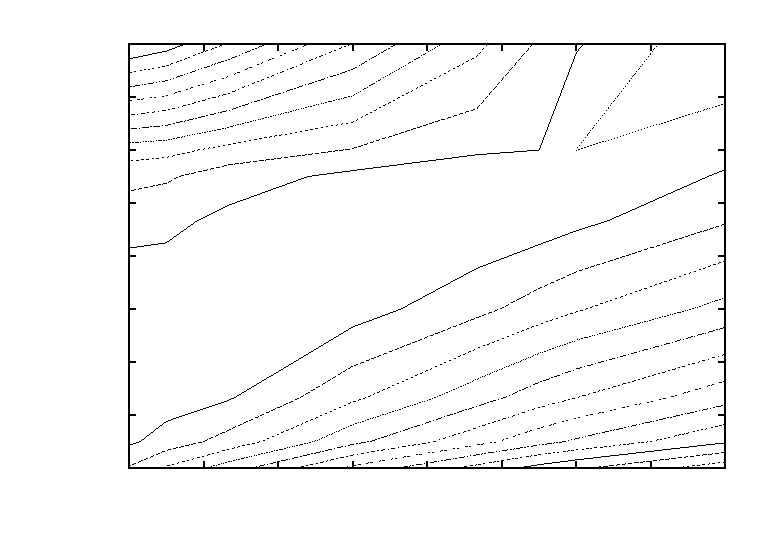
\includegraphics{chapters/chapter6/desertantplot}}%
    \gplfronttext
  \end{picture}%
\endgroup
}
\caption{Contour plot of values for $\sigma$ over values for $r$ and $\tau$ for desert ant foraging}
\label{desertantplot}
\end{figure}


%\begin{figure}
%\input{naiveplot.tex}
%\caption{Contour plot of values for $\sigma$ over values for $r$ and $\tau$ for nai%\"ve foraging}
%\end{figure}

 %But why? Give reason 
%The nai\"ve foraging algorithm slowly clear an entire area around the sink. If there is an equal ratio of robot types to item types then this area would be cleared effectively. 
 %fact that in the more organized environments such as gaussian or vein, it is 

\subsubsection{Independence of the Honey Bee Foraging Algorithm to Item Type Ratio}
\label{Adaptability}

Analysis of Table \ref{ratio} indicates that the honey bee foraging algorithm has similar performance throughout all configurations for $r$ and $\tau$, which highlights that the performance of the honey bee algorithm is independent of the configuration of $\tau$, thus one can conclude that the honey bee algorithm is more flexible and robust. This could mean that the honey bee algorithm could perform well in dynamic environments where robots and items can be destroyed.

However, according to Table \ref{ratio}, the desert ant algorithm performs better than the honey bee algorithm, for particular configurations of $r$ and $\tau$. This indicates that, if the value of $r$ is known for a particular environment, then it is beneficial to use desert ant foraging and choose $\tau$ appropriately. A possible reason why the desert ant algorithm performs better when optimally configured for a particular environment than the honey bee algorithm is that the honey bee algorithm takes time to adapt to the environment, while the desert ant algorithm with optimal configurations has no division of labour overhead and may outperform the honey bee algorithm under those circumstances.

\subsection{Environment Types}
\label{results:environmentaltypes}

\begin{table} [h]
     \caption{Prioritized Items over time over different Environment Types for each Algorithm}
     \label{ratio}
	\centering
	\footnotesize
	\begin{tabular} {|l|l|l|l|}
\hline
name & Naive & DesertAnt & HoneyBee \\
\hline
clustered & 0.414017 (0.388334)  & 0.504665 (0.396114)  & 0.537091 (0.378332)  \\
gaussian & 0.389998 (0.403603)  & 0.487472 (0.416113)  & 0.542252 (0.399359)  \\
uniform & 0.413511 (0.388773)  & 0.502372 (0.395749)  & 0.530851 (0.376446)  \\
vein & 0.370908 (0.401867)  & 0.482342 (0.419204)  & 0.54274 (0.408115)  \\
\hline
\end{tabular}

\end{table}


\begin{figure}[!htb]
\centering
\resizebox{0.8\textwidth}{!}{% GNUPLOT: LaTeX picture with Postscript
\begingroup
  \makeatletter
  \providecommand\color[2][]{%
    \GenericError{(gnuplot) \space\space\space\@spaces}{%
      Package color not loaded in conjunction with
      terminal option `colourtext'%
    }{See the gnuplot documentation for explanation.%
    }{Either use 'blacktext' in gnuplot or load the package
      color.sty in LaTeX.}%
    \renewcommand\color[2][]{}%
  }%
  \providecommand\includegraphics[2][]{%
    \GenericError{(gnuplot) \space\space\space\@spaces}{%
      Package graphicx or graphics not loaded%
    }{See the gnuplot documentation for explanation.%
    }{The gnuplot epslatex terminal needs graphicx.sty or graphics.sty.}%
    \renewcommand\includegraphics[2][]{}%
  }%
  \providecommand\rotatebox[2]{#2}%
  \@ifundefined{ifGPcolor}{%
    \newif\ifGPcolor
    \GPcolorfalse
  }{}%
  \@ifundefined{ifGPblacktext}{%
    \newif\ifGPblacktext
    \GPblacktexttrue
  }{}%
  % define a \g@addto@macro without @ in the name:
  \let\gplgaddtomacro\g@addto@macro
  % define empty templates for all commands taking text:
  \gdef\gplbacktext{}%
  \gdef\gplfronttext{}%
  \makeatother
  \ifGPblacktext
    % no textcolor at all
    \def\colorrgb#1{}%
    \def\colorgray#1{}%
  \else
    % gray or color?
    \ifGPcolor
      \def\colorrgb#1{\color[rgb]{#1}}%
      \def\colorgray#1{\color[gray]{#1}}%
      \expandafter\def\csname LTw\endcsname{\color{white}}%
      \expandafter\def\csname LTb\endcsname{\color{black}}%
      \expandafter\def\csname LTa\endcsname{\color{black}}%
      \expandafter\def\csname LT0\endcsname{\color[rgb]{1,0,0}}%
      \expandafter\def\csname LT1\endcsname{\color[rgb]{0,1,0}}%
      \expandafter\def\csname LT2\endcsname{\color[rgb]{0,0,1}}%
      \expandafter\def\csname LT3\endcsname{\color[rgb]{1,0,1}}%
      \expandafter\def\csname LT4\endcsname{\color[rgb]{0,1,1}}%
      \expandafter\def\csname LT5\endcsname{\color[rgb]{1,1,0}}%
      \expandafter\def\csname LT6\endcsname{\color[rgb]{0,0,0}}%
      \expandafter\def\csname LT7\endcsname{\color[rgb]{1,0.3,0}}%
      \expandafter\def\csname LT8\endcsname{\color[rgb]{0.5,0.5,0.5}}%
    \else
      % gray
      \def\colorrgb#1{\color{black}}%
      \def\colorgray#1{\color[gray]{#1}}%
      \expandafter\def\csname LTw\endcsname{\color{white}}%
      \expandafter\def\csname LTb\endcsname{\color{black}}%
      \expandafter\def\csname LTa\endcsname{\color{black}}%
      \expandafter\def\csname LT0\endcsname{\color{black}}%
      \expandafter\def\csname LT1\endcsname{\color{black}}%
      \expandafter\def\csname LT2\endcsname{\color{black}}%
      \expandafter\def\csname LT3\endcsname{\color{black}}%
      \expandafter\def\csname LT4\endcsname{\color{black}}%
      \expandafter\def\csname LT5\endcsname{\color{black}}%
      \expandafter\def\csname LT6\endcsname{\color{black}}%
      \expandafter\def\csname LT7\endcsname{\color{black}}%
      \expandafter\def\csname LT8\endcsname{\color{black}}%
    \fi
  \fi
    \setlength{\unitlength}{0.0500bp}%
    \ifx\gptboxheight\undefined%
      \newlength{\gptboxheight}%
      \newlength{\gptboxwidth}%
      \newsavebox{\gptboxtext}%
    \fi%
    \setlength{\fboxrule}{0.5pt}%
    \setlength{\fboxsep}{1pt}%
\begin{picture}(7200.00,5040.00)%
    \gplgaddtomacro\gplbacktext{%
      \csname LTb\endcsname%
      \put(594,440){\makebox(0,0)[r]{\strut{}$0$}}%
      \put(594,982){\makebox(0,0)[r]{\strut{}$0.1$}}%
      \put(594,1524){\makebox(0,0)[r]{\strut{}$0.2$}}%
      \put(594,2066){\makebox(0,0)[r]{\strut{}$0.3$}}%
      \put(594,2608){\makebox(0,0)[r]{\strut{}$0.4$}}%
      \put(594,3149){\makebox(0,0)[r]{\strut{}$0.5$}}%
      \put(594,3691){\makebox(0,0)[r]{\strut{}$0.6$}}%
      \put(594,4233){\makebox(0,0)[r]{\strut{}$0.7$}}%
      \put(594,4775){\makebox(0,0)[r]{\strut{}$0.8$}}%
      \put(2245,220){\makebox(0,0){\strut{}Na\"ive}}%
      \put(3765,220){\makebox(0,0){\strut{}DesertAnt}}%
      \put(5284,220){\makebox(0,0){\strut{}HoneyBee}}%
    }%
    \gplgaddtomacro\gplfronttext{%
      \csname LTb\endcsname%
      \put(5816,4602){\makebox(0,0)[r]{\strut{}Uniform}}%
      \csname LTb\endcsname%
      \put(5816,4382){\makebox(0,0)[r]{\strut{}Clustered}}%
      \csname LTb\endcsname%
      \put(5816,4162){\makebox(0,0)[r]{\strut{}Gaussian}}%
      \csname LTb\endcsname%
      \put(5816,3942){\makebox(0,0)[r]{\strut{}Vein}}%
    }%
    \gplbacktext
    \put(0,0){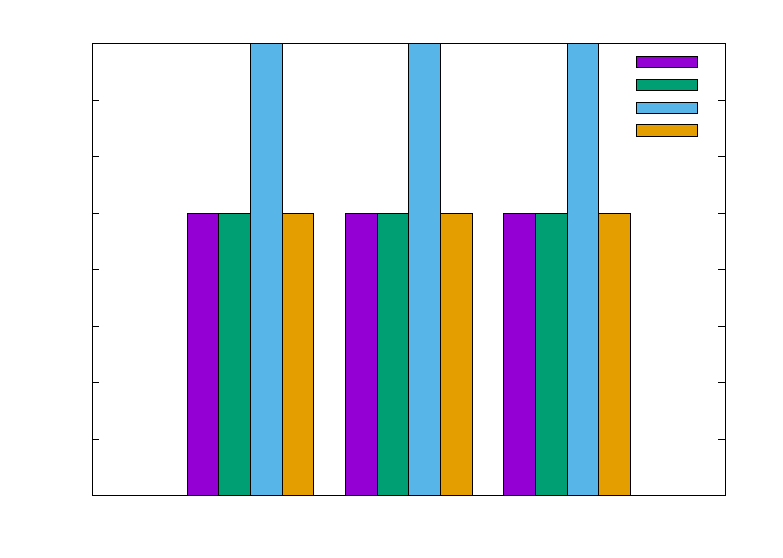
\includegraphics{chapters/chapter6/graphs/environment_types}}%
    \gplfronttext
  \end{picture}%
\endgroup
}
\caption{Prioritized Items over time over different Environment Types for each Algorithm}
\label{environmenttypes}
\end{figure}


It is possible that the algorithms will perform differently on different types of environments by exploiting their capabilities to memorize and communicate the location of areas with a high prioritized item density or conversely by using their exploration abilities to find new items. The performance of the algorithms is analysed over the different types of environments. The following hypotheses are explored:  

\begin{enumerate}
	\item The na\"ive foraging algorithm will perform better on environments with a uniform distribution compared to the clustered, the vein and Gaussian environments, due to the algorithms inability to return to areas with high item density. 
	\item The desert ant foraging algorithm will perform better on clustered, Gaussian and vein environments environments due to their capability to remember locations and thus are able to return quickly to areas that are rich in prioritized items.
	 \item The honey bee foraging algorithm will perform best on Gaussian distribution environments since it will be able to recruit members to explore and forage even quicker than the desert ant. Honey bee will likely perform worse on the uniformly distributed environments as there may be time wasted to recruit robots to areas which do not especially contain prioritized items.
\end{enumerate}

\begin{figure}[!htb]
\centering
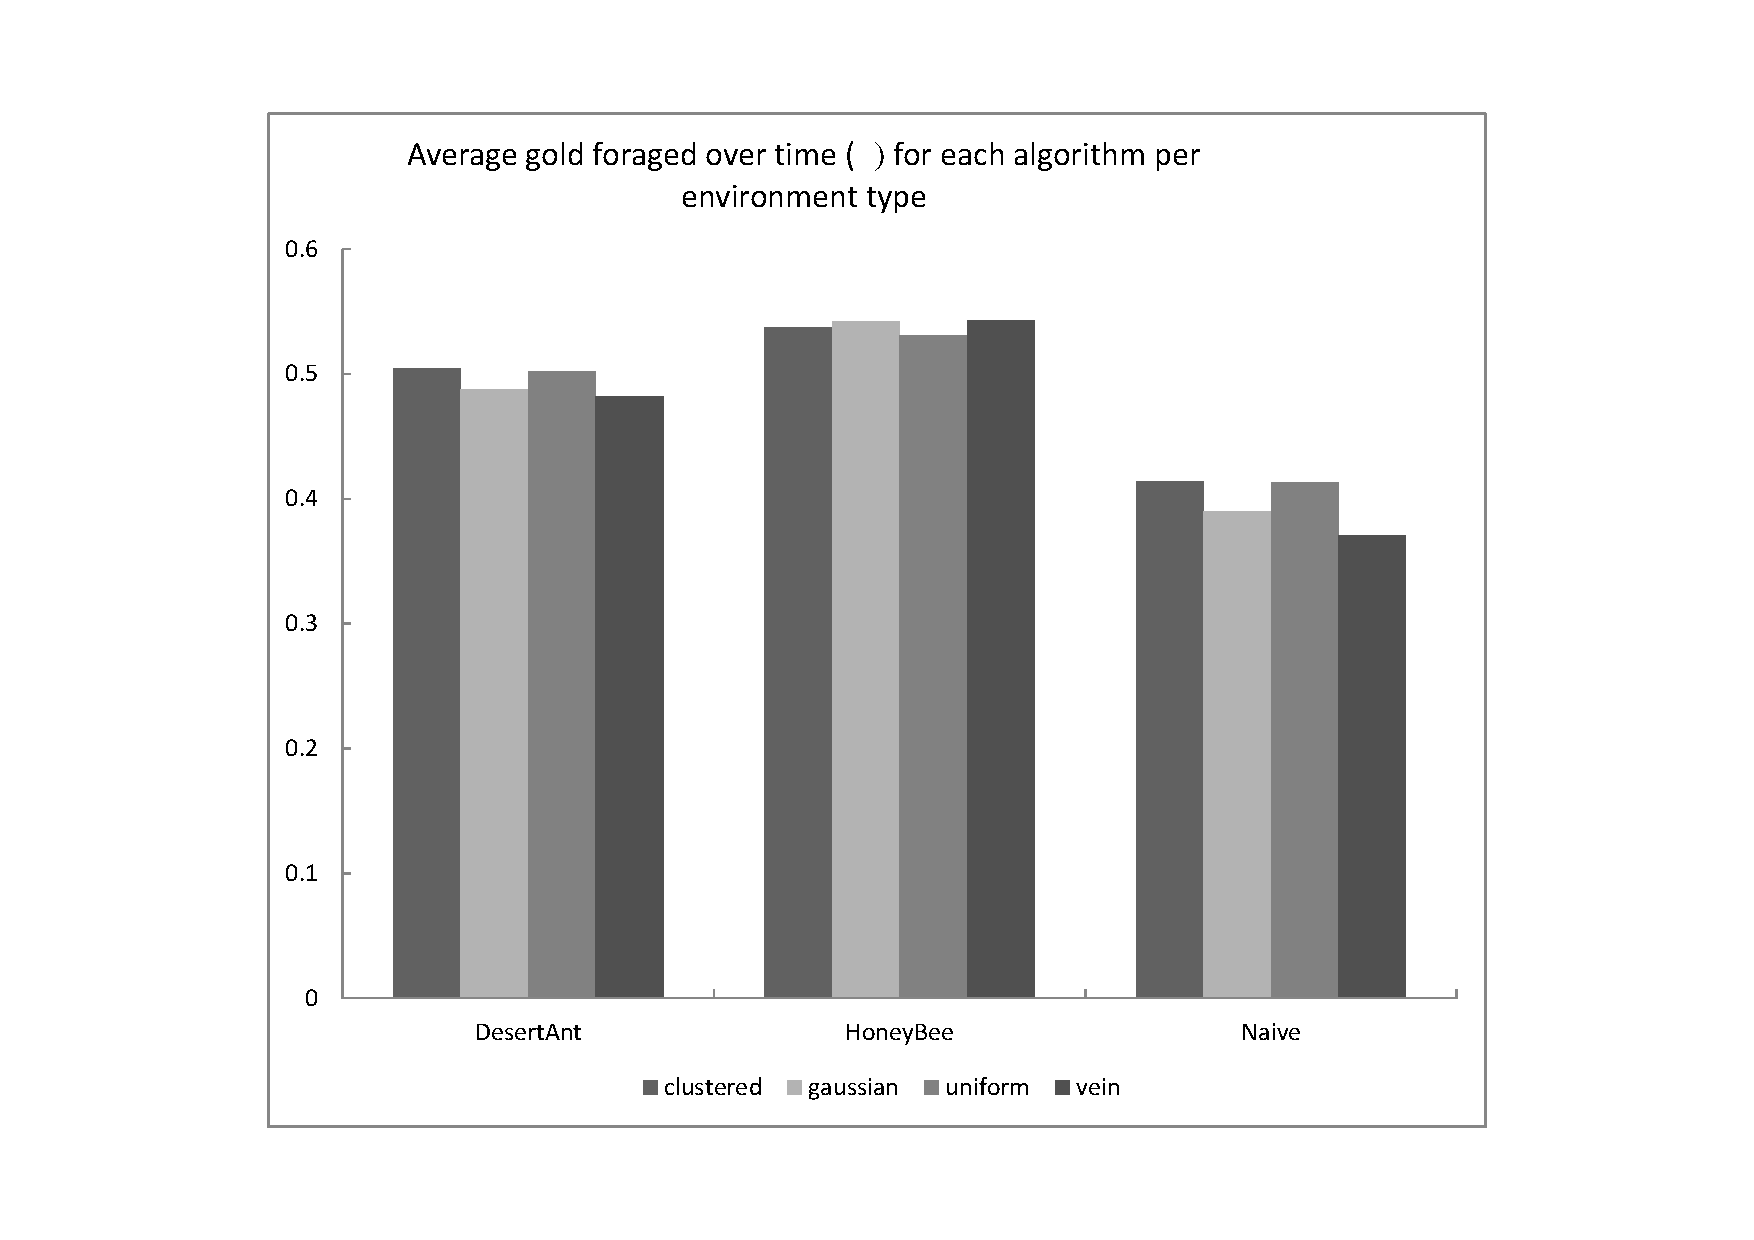
\includegraphics[width=\textwidth]{chapters/chapter6/graphs/gold_environment.pdf}
\caption{Prioritized items over time per environment type for each algorithm}
\label{environmentgoldplot}
\end{figure}
%TODO: Insert graph and table from new results.
By examining table X and graph Y, it is clear that suprisingly the environment types have less of an effect on performance ($\sigma$ and $\mu$) than expected thus one can conclude that the algorithms either do not effectively take advantage of some of the environment types or do take advantage of environment types but are hindered by other difficulties related to the environment type. Another general and suprising notion across all environments is that performance of the algorithm over clustered environments seems to be similar performance of the algorithms over uniform environments. This is unexpected since, due to the fact that the clustered environment has grouped areas of prioritized items, one would expect the performance of algorithms over clustered environments to be more similar to the performance of algorithms over vein and gaussian environments since vein and gaussian environments also have grouped areas of prioritized items. The conclusion after examining a number of the environments is that the generated clustered environments do not have sparsely defined clusters and thus the clustered environments are perhaps more similar to the uniform environments. 

As expected, the na\"ive algorithm performs the best on uniform environments and the worst on gaussian and vein environments. As discussed above, the na\"ive algorithm also performs similarly on the clustered environments as it does on the uniform environments, but besides that anomaly, the first hypothesis about na\"ive environments is confirmed. 

Table x and graph Y surpisingly do not confirm the second hypothesis that the desert ant algorithm will perform better on the gaussian and vein environments than the uniform environments. The reason for this is actually obvious after careful thought. The uniform environment can be considered a simpler environment type than the  clustered, gaussian and vein environments since the uniform environment is less likely to result in large areas of non-prioritized items that may form larger obstacles that are difficult to navigate around. Not only that, but the uniform distribution will result in less robot-to-robot interference than gaussian and vein environments since the robots are not all trying to navigate towards the same area to locate the items and are thus likely to be evenly spread across the environment. Unlike the honey bee algorithm, which may actively be at a disadvantage in a uniform environment due to potential overhead from division of labour between foraging and resting robots and the specialization ratio division of labour, the desert ant algorithm has no such overhead. Due to the simpler nature of the uniform environment, it is thus not suprising that the desert ant algorithm performs better on the uniform environment as opposed to the more difficult vein and gaussian environments. As discussed above, the desert ant algorithm performed similarly on clustered environments as it did on uniform environments. 

The honey bee algorithm performs as expected, performing better on gaussian and environments and worse on the clustered and uniform environments. As stated above, the honey bee algorthim is actively hindered in uniform environments as it may falsely detect that the location of an environment is worth broadcasting to other robots, and thus robots are unnecessarily recruited to an area which does not have a rich concentration of prioritized items. The other problem is that there may be overhead where robots falsely switch between foraging prioritized and non-prioritized items when falsely detecting that a switch is required and thus robots end up thrashing back and forth between foraging prioritized and non-prioritized items. The honey bee algorithm is thus more suited to environments which has areas of higher concentrations of particular types of items so that division of labour does not cause unnecessary overhead and instead benefits the performance of the algorithm. 

\subsection{Item Density}
\label{results:itemdensity}

\begin{table} [h]
     \caption{Prioritized Items over Time over Item Density in Environment for each Algorithm}
     \label{ratio}
	\centering
	\footnotesize
	\begin{tabular} {|l|l|l|l|}
\hline
$p$ & Naive & DesertAnt & HoneyBee \\
\hline
0.05 & 0.58576 (0.397434)  & 0.709257 (0.370191)  & 0.724892 (0.331663)  \\
0.2 & 0.445301 (0.400194)  & 0.55749 (0.396821)  & 0.601527 (0.374943)  \\
0.5 & 0.34856 (0.3778)  & 0.441694 (0.395469)  & 0.494143 (0.388125)  \\
0.7 & 0.315063 (0.368166)  & 0.396919 (0.389359)  & 0.451818 (0.388338)  \\
0.9 & 0.290859 (0.360364)  & 0.365705 (0.383365)  & 0.418788 (0.38623)  \\
\hline
\end{tabular}

\end{table}


\begin{figure}[!htb]
\centering
\resizebox{\textwidth}{!}{% GNUPLOT: LaTeX picture with Postscript
\begingroup
  \makeatletter
  \providecommand\color[2][]{%
    \GenericError{(gnuplot) \space\space\space\@spaces}{%
      Package color not loaded in conjunction with
      terminal option `colourtext'%
    }{See the gnuplot documentation for explanation.%
    }{Either use 'blacktext' in gnuplot or load the package
      color.sty in LaTeX.}%
    \renewcommand\color[2][]{}%
  }%
  \providecommand\includegraphics[2][]{%
    \GenericError{(gnuplot) \space\space\space\@spaces}{%
      Package graphicx or graphics not loaded%
    }{See the gnuplot documentation for explanation.%
    }{The gnuplot epslatex terminal needs graphicx.sty or graphics.sty.}%
    \renewcommand\includegraphics[2][]{}%
  }%
  \providecommand\rotatebox[2]{#2}%
  \@ifundefined{ifGPcolor}{%
    \newif\ifGPcolor
    \GPcolorfalse
  }{}%
  \@ifundefined{ifGPblacktext}{%
    \newif\ifGPblacktext
    \GPblacktexttrue
  }{}%
  % define a \g@addto@macro without @ in the name:
  \let\gplgaddtomacro\g@addto@macro
  % define empty templates for all commands taking text:
  \gdef\gplbacktext{}%
  \gdef\gplfronttext{}%
  \makeatother
  \ifGPblacktext
    % no textcolor at all
    \def\colorrgb#1{}%
    \def\colorgray#1{}%
  \else
    % gray or color?
    \ifGPcolor
      \def\colorrgb#1{\color[rgb]{#1}}%
      \def\colorgray#1{\color[gray]{#1}}%
      \expandafter\def\csname LTw\endcsname{\color{white}}%
      \expandafter\def\csname LTb\endcsname{\color{black}}%
      \expandafter\def\csname LTa\endcsname{\color{black}}%
      \expandafter\def\csname LT0\endcsname{\color[rgb]{1,0,0}}%
      \expandafter\def\csname LT1\endcsname{\color[rgb]{0,1,0}}%
      \expandafter\def\csname LT2\endcsname{\color[rgb]{0,0,1}}%
      \expandafter\def\csname LT3\endcsname{\color[rgb]{1,0,1}}%
      \expandafter\def\csname LT4\endcsname{\color[rgb]{0,1,1}}%
      \expandafter\def\csname LT5\endcsname{\color[rgb]{1,1,0}}%
      \expandafter\def\csname LT6\endcsname{\color[rgb]{0,0,0}}%
      \expandafter\def\csname LT7\endcsname{\color[rgb]{1,0.3,0}}%
      \expandafter\def\csname LT8\endcsname{\color[rgb]{0.5,0.5,0.5}}%
    \else
      % gray
      \def\colorrgb#1{\color{black}}%
      \def\colorgray#1{\color[gray]{#1}}%
      \expandafter\def\csname LTw\endcsname{\color{white}}%
      \expandafter\def\csname LTb\endcsname{\color{black}}%
      \expandafter\def\csname LTa\endcsname{\color{black}}%
      \expandafter\def\csname LT0\endcsname{\color{black}}%
      \expandafter\def\csname LT1\endcsname{\color{black}}%
      \expandafter\def\csname LT2\endcsname{\color{black}}%
      \expandafter\def\csname LT3\endcsname{\color{black}}%
      \expandafter\def\csname LT4\endcsname{\color{black}}%
      \expandafter\def\csname LT5\endcsname{\color{black}}%
      \expandafter\def\csname LT6\endcsname{\color{black}}%
      \expandafter\def\csname LT7\endcsname{\color{black}}%
      \expandafter\def\csname LT8\endcsname{\color{black}}%
    \fi
  \fi
  \setlength{\unitlength}{0.0500bp}%
  \begin{picture}(7200.00,5040.00)%
    \gplgaddtomacro\gplbacktext{%
      \csname LTb\endcsname%
      \put(1078,704){\makebox(0,0)[r]{\strut{} 0.25}}%
      \put(1078,1071){\makebox(0,0)[r]{\strut{} 0.3}}%
      \put(1078,1439){\makebox(0,0)[r]{\strut{} 0.35}}%
      \put(1078,1806){\makebox(0,0)[r]{\strut{} 0.4}}%
      \put(1078,2174){\makebox(0,0)[r]{\strut{} 0.45}}%
      \put(1078,2541){\makebox(0,0)[r]{\strut{} 0.5}}%
      \put(1078,2909){\makebox(0,0)[r]{\strut{} 0.55}}%
      \put(1078,3276){\makebox(0,0)[r]{\strut{} 0.6}}%
      \put(1078,3644){\makebox(0,0)[r]{\strut{} 0.65}}%
      \put(1078,4012){\makebox(0,0)[r]{\strut{} 0.7}}%
      \put(1078,4379){\makebox(0,0)[r]{\strut{} 0.75}}%
      \put(1210,484){\makebox(0,0){\strut{} 0}}%
      \put(1831,484){\makebox(0,0){\strut{} 0.1}}%
      \put(2453,484){\makebox(0,0){\strut{} 0.2}}%
      \put(3074,484){\makebox(0,0){\strut{} 0.3}}%
      \put(3696,484){\makebox(0,0){\strut{} 0.4}}%
      \put(4317,484){\makebox(0,0){\strut{} 0.5}}%
      \put(4939,484){\makebox(0,0){\strut{} 0.6}}%
      \put(5560,484){\makebox(0,0){\strut{} 0.7}}%
      \put(6182,484){\makebox(0,0){\strut{} 0.8}}%
      \put(6803,484){\makebox(0,0){\strut{} 0.9}}%
      \put(176,2541){\rotatebox{-270}{\makebox(0,0){\strut{}Prioritized items over time ($\sigma$)}}}%
      \put(4006,154){\makebox(0,0){\strut{}Amount of Objects ($p$)}}%
      \put(4006,4709){\makebox(0,0){\strut{}Prioritized items over time for each algorithm over item density}}%
    }%
    \gplgaddtomacro\gplfronttext{%
      \csname LTb\endcsname%
      \put(5816,4206){\makebox(0,0)[r]{\strut{}Na\"ive}}%
      \csname LTb\endcsname%
      \put(5816,3986){\makebox(0,0)[r]{\strut{}Desert Ant}}%
      \csname LTb\endcsname%
      \put(5816,3766){\makebox(0,0)[r]{\strut{}Honey Bee}}%
    }%
    \gplbacktext
    \put(0,0){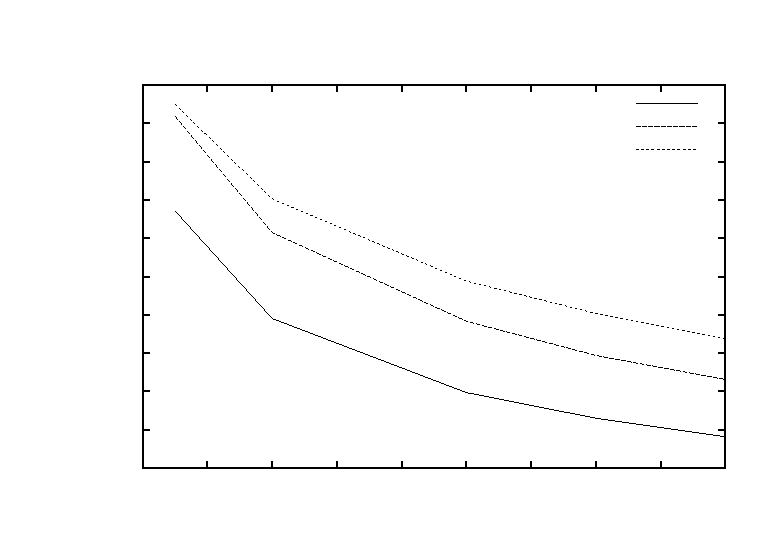
\includegraphics{chapters/chapter6/graphs/gold_objects}}%
    \gplfronttext
  \end{picture}%
\endgroup
}
\caption{Prioritized Items over Time over Item Density in Environment  for each Algorithm}
\label{objectgoldplot}
\end{figure}


\begin{figure}[!htb]
\centering
\resizebox{\textwidth}{!}{% GNUPLOT: LaTeX picture with Postscript
\begingroup
  \makeatletter
  \providecommand\color[2][]{%
    \GenericError{(gnuplot) \space\space\space\@spaces}{%
      Package color not loaded in conjunction with
      terminal option `colourtext'%
    }{See the gnuplot documentation for explanation.%
    }{Either use 'blacktext' in gnuplot or load the package
      color.sty in LaTeX.}%
    \renewcommand\color[2][]{}%
  }%
  \providecommand\includegraphics[2][]{%
    \GenericError{(gnuplot) \space\space\space\@spaces}{%
      Package graphicx or graphics not loaded%
    }{See the gnuplot documentation for explanation.%
    }{The gnuplot epslatex terminal needs graphicx.sty or graphics.sty.}%
    \renewcommand\includegraphics[2][]{}%
  }%
  \providecommand\rotatebox[2]{#2}%
  \@ifundefined{ifGPcolor}{%
    \newif\ifGPcolor
    \GPcolorfalse
  }{}%
  \@ifundefined{ifGPblacktext}{%
    \newif\ifGPblacktext
    \GPblacktexttrue
  }{}%
  % define a \g@addto@macro without @ in the name:
  \let\gplgaddtomacro\g@addto@macro
  % define empty templates for all commands taking text:
  \gdef\gplbacktext{}%
  \gdef\gplfronttext{}%
  \makeatother
  \ifGPblacktext
    % no textcolor at all
    \def\colorrgb#1{}%
    \def\colorgray#1{}%
  \else
    % gray or color?
    \ifGPcolor
      \def\colorrgb#1{\color[rgb]{#1}}%
      \def\colorgray#1{\color[gray]{#1}}%
      \expandafter\def\csname LTw\endcsname{\color{white}}%
      \expandafter\def\csname LTb\endcsname{\color{black}}%
      \expandafter\def\csname LTa\endcsname{\color{black}}%
      \expandafter\def\csname LT0\endcsname{\color[rgb]{1,0,0}}%
      \expandafter\def\csname LT1\endcsname{\color[rgb]{0,1,0}}%
      \expandafter\def\csname LT2\endcsname{\color[rgb]{0,0,1}}%
      \expandafter\def\csname LT3\endcsname{\color[rgb]{1,0,1}}%
      \expandafter\def\csname LT4\endcsname{\color[rgb]{0,1,1}}%
      \expandafter\def\csname LT5\endcsname{\color[rgb]{1,1,0}}%
      \expandafter\def\csname LT6\endcsname{\color[rgb]{0,0,0}}%
      \expandafter\def\csname LT7\endcsname{\color[rgb]{1,0.3,0}}%
      \expandafter\def\csname LT8\endcsname{\color[rgb]{0.5,0.5,0.5}}%
    \else
      % gray
      \def\colorrgb#1{\color{black}}%
      \def\colorgray#1{\color[gray]{#1}}%
      \expandafter\def\csname LTw\endcsname{\color{white}}%
      \expandafter\def\csname LTb\endcsname{\color{black}}%
      \expandafter\def\csname LTa\endcsname{\color{black}}%
      \expandafter\def\csname LT0\endcsname{\color{black}}%
      \expandafter\def\csname LT1\endcsname{\color{black}}%
      \expandafter\def\csname LT2\endcsname{\color{black}}%
      \expandafter\def\csname LT3\endcsname{\color{black}}%
      \expandafter\def\csname LT4\endcsname{\color{black}}%
      \expandafter\def\csname LT5\endcsname{\color{black}}%
      \expandafter\def\csname LT6\endcsname{\color{black}}%
      \expandafter\def\csname LT7\endcsname{\color{black}}%
      \expandafter\def\csname LT8\endcsname{\color{black}}%
    \fi
  \fi
  \setlength{\unitlength}{0.0500bp}%
  \begin{picture}(7200.00,5040.00)%
    \gplgaddtomacro\gplbacktext{%
      \csname LTb\endcsname%
      \put(946,704){\makebox(0,0)[r]{\strut{} 0.3}}%
      \put(946,1229){\makebox(0,0)[r]{\strut{} 0.4}}%
      \put(946,1754){\makebox(0,0)[r]{\strut{} 0.5}}%
      \put(946,2279){\makebox(0,0)[r]{\strut{} 0.6}}%
      \put(946,2804){\makebox(0,0)[r]{\strut{} 0.7}}%
      \put(946,3329){\makebox(0,0)[r]{\strut{} 0.8}}%
      \put(946,3854){\makebox(0,0)[r]{\strut{} 0.9}}%
      \put(946,4379){\makebox(0,0)[r]{\strut{} 1}}%
      \put(1078,484){\makebox(0,0){\strut{} 0}}%
      \put(2223,484){\makebox(0,0){\strut{} 0.2}}%
      \put(3368,484){\makebox(0,0){\strut{} 0.4}}%
      \put(4513,484){\makebox(0,0){\strut{} 0.6}}%
      \put(5658,484){\makebox(0,0){\strut{} 0.8}}%
      \put(6803,484){\makebox(0,0){\strut{} 1}}%
      \put(176,2541){\rotatebox{-270}{\makebox(0,0){\strut{}Non-prioritized items over time ($\sigma$)}}}%
      \put(3940,154){\makebox(0,0){\strut{}Amount of Objects ($p$)}}%
      \put(3940,4709){\makebox(0,0){\strut{}Non-prioritized items over time for each algorithm over object percentages}}%
    }%
    \gplgaddtomacro\gplfronttext{%
      \csname LTb\endcsname%
      \put(5816,4206){\makebox(0,0)[r]{\strut{}Na\"ive}}%
      \csname LTb\endcsname%
      \put(5816,3986){\makebox(0,0)[r]{\strut{}Desert Ant}}%
      \csname LTb\endcsname%
      \put(5816,3766){\makebox(0,0)[r]{\strut{}Honey Bee}}%
    }%
    \gplbacktext
    \put(0,0){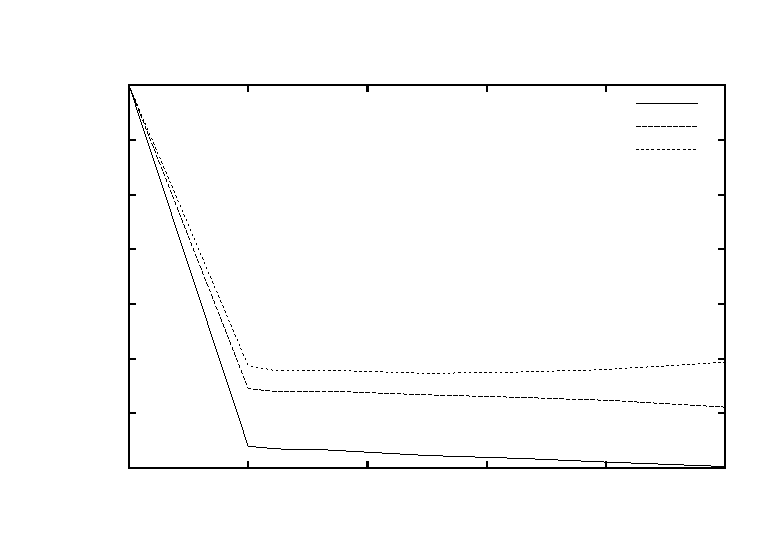
\includegraphics{chapters/chapter6/graphs/waste_objects}}%
    \gplfronttext
  \end{picture}%
\endgroup
}
\caption{Non-prioritized Items over Time over Item Density in Environment for each Algorithm}
\label{objectwasteplot}
\end{figure}

Item density is examined in order to determine if algorithm performance is affected y an increase in environment complexity. As the density of items increases, the more difficult navigation becomes around non-prioritized items that form obstalces when there isn't a suitable specialization ratio of robots. Conversely however, the more dense the enviroment's are then the richer and denser the deposits of prioritized items may becomes in certain environments, thus the division of labour of the honey bee algorithm may become more effective at higher densities. As indicated in \ref{objectgoldplot}, all algorithms are shown to degrade quite heavily as the items density increases. This is to be expected as it will take longer for robots to forage all items in the denser environment. Thus the degradation of performance can likely be attributed to the limit on simulation time which should have been extended in order to cater for the large environments. Unfortunately, to adequately compare and analyse the performance as item density increases, one would have to allow more time over all to simulations.

\section{Robustness}
\label{results:robustness}

Robustness can be defined as an algorithms ability to degrade gracefully or recover from damage or mulfunction of a portion of the swarm. A robust algorithms performance should thus be independant of any specific initial swarm configuration such as the specialization ratio. The more homogenous the swarm, in general, the more robust the swarm will be to failure of a portion of the swarm since the swarm will not have any dependancies on a specific individual or group of individuals within the swarm. The less homogenous the swarm is, the most likely the swarm will suffer when individuals with specific capabilities malfunction or are damaged.

\subsection{Specialization}
\label{results:specialization}

The reason the initial robot specialization has been included under robustness is that the more dependant the algorithm is to robot specialization, the more sensitive  the algorithm is to robots becoming damaged. When referring to specialization in this chpater, it is referring specifically to the initial specialization ratio $\tau$ of the swarm of robots. 

\begin{figure}[!htb]
\centering
\resizebox{\textwidth}{!}{% GNUPLOT: LaTeX picture with Postscript
\begingroup
  \makeatletter
  \providecommand\color[2][]{%
    \GenericError{(gnuplot) \space\space\space\@spaces}{%
      Package color not loaded in conjunction with
      terminal option `colourtext'%
    }{See the gnuplot documentation for explanation.%
    }{Either use 'blacktext' in gnuplot or load the package
      color.sty in LaTeX.}%
    \renewcommand\color[2][]{}%
  }%
  \providecommand\includegraphics[2][]{%
    \GenericError{(gnuplot) \space\space\space\@spaces}{%
      Package graphicx or graphics not loaded%
    }{See the gnuplot documentation for explanation.%
    }{The gnuplot epslatex terminal needs graphicx.sty or graphics.sty.}%
    \renewcommand\includegraphics[2][]{}%
  }%
  \providecommand\rotatebox[2]{#2}%
  \@ifundefined{ifGPcolor}{%
    \newif\ifGPcolor
    \GPcolorfalse
  }{}%
  \@ifundefined{ifGPblacktext}{%
    \newif\ifGPblacktext
    \GPblacktexttrue
  }{}%
  % define a \g@addto@macro without @ in the name:
  \let\gplgaddtomacro\g@addto@macro
  % define empty templates for all commands taking text:
  \gdef\gplbacktext{}%
  \gdef\gplfronttext{}%
  \makeatother
  \ifGPblacktext
    % no textcolor at all
    \def\colorrgb#1{}%
    \def\colorgray#1{}%
  \else
    % gray or color?
    \ifGPcolor
      \def\colorrgb#1{\color[rgb]{#1}}%
      \def\colorgray#1{\color[gray]{#1}}%
      \expandafter\def\csname LTw\endcsname{\color{white}}%
      \expandafter\def\csname LTb\endcsname{\color{black}}%
      \expandafter\def\csname LTa\endcsname{\color{black}}%
      \expandafter\def\csname LT0\endcsname{\color[rgb]{1,0,0}}%
      \expandafter\def\csname LT1\endcsname{\color[rgb]{0,1,0}}%
      \expandafter\def\csname LT2\endcsname{\color[rgb]{0,0,1}}%
      \expandafter\def\csname LT3\endcsname{\color[rgb]{1,0,1}}%
      \expandafter\def\csname LT4\endcsname{\color[rgb]{0,1,1}}%
      \expandafter\def\csname LT5\endcsname{\color[rgb]{1,1,0}}%
      \expandafter\def\csname LT6\endcsname{\color[rgb]{0,0,0}}%
      \expandafter\def\csname LT7\endcsname{\color[rgb]{1,0.3,0}}%
      \expandafter\def\csname LT8\endcsname{\color[rgb]{0.5,0.5,0.5}}%
    \else
      % gray
      \def\colorrgb#1{\color{black}}%
      \def\colorgray#1{\color[gray]{#1}}%
      \expandafter\def\csname LTw\endcsname{\color{white}}%
      \expandafter\def\csname LTb\endcsname{\color{black}}%
      \expandafter\def\csname LTa\endcsname{\color{black}}%
      \expandafter\def\csname LT0\endcsname{\color{black}}%
      \expandafter\def\csname LT1\endcsname{\color{black}}%
      \expandafter\def\csname LT2\endcsname{\color{black}}%
      \expandafter\def\csname LT3\endcsname{\color{black}}%
      \expandafter\def\csname LT4\endcsname{\color{black}}%
      \expandafter\def\csname LT5\endcsname{\color{black}}%
      \expandafter\def\csname LT6\endcsname{\color{black}}%
      \expandafter\def\csname LT7\endcsname{\color{black}}%
      \expandafter\def\csname LT8\endcsname{\color{black}}%
    \fi
  \fi
  \setlength{\unitlength}{0.0500bp}%
  \begin{picture}(7200.00,5040.00)%
    \gplgaddtomacro\gplbacktext{%
      \csname LTb\endcsname%
      \put(1078,704){\makebox(0,0)[r]{\strut{} 0.1}}%
      \put(1078,1072){\makebox(0,0)[r]{\strut{} 0.15}}%
      \put(1078,1439){\makebox(0,0)[r]{\strut{} 0.2}}%
      \put(1078,1806){\makebox(0,0)[r]{\strut{} 0.25}}%
      \put(1078,2174){\makebox(0,0)[r]{\strut{} 0.3}}%
      \put(1078,2541){\makebox(0,0)[r]{\strut{} 0.35}}%
      \put(1078,2909){\makebox(0,0)[r]{\strut{} 0.4}}%
      \put(1078,3276){\makebox(0,0)[r]{\strut{} 0.45}}%
      \put(1078,3644){\makebox(0,0)[r]{\strut{} 0.5}}%
      \put(1078,4011){\makebox(0,0)[r]{\strut{} 0.55}}%
      \put(1078,4379){\makebox(0,0)[r]{\strut{} 0.6}}%
      \put(1210,484){\makebox(0,0){\strut{} 0}}%
      \put(2329,484){\makebox(0,0){\strut{} 0.2}}%
      \put(3447,484){\makebox(0,0){\strut{} 0.4}}%
      \put(4566,484){\makebox(0,0){\strut{} 0.6}}%
      \put(5684,484){\makebox(0,0){\strut{} 0.8}}%
      \put(6803,484){\makebox(0,0){\strut{} 1}}%
      \put(176,2541){\rotatebox{-270}{\makebox(0,0){\strut{}Prioritized items over time ($\sigma$)}}}%
      \put(4006,154){\makebox(0,0){\strut{}Robot Type Ratio ($r$)}}%
      \put(4006,4709){\makebox(0,0){\strut{}Prioritized items over time for each algorithm for robot type ratios}}%
    }%
    \gplgaddtomacro\gplfronttext{%
      \csname LTb\endcsname%
      \put(5816,4206){\makebox(0,0)[r]{\strut{}Na\"ive}}%
      \csname LTb\endcsname%
      \put(5816,3986){\makebox(0,0)[r]{\strut{}Desert Ant}}%
      \csname LTb\endcsname%
      \put(5816,3766){\makebox(0,0)[r]{\strut{}Honey Bee}}%
    }%
    \gplbacktext
    \put(0,0){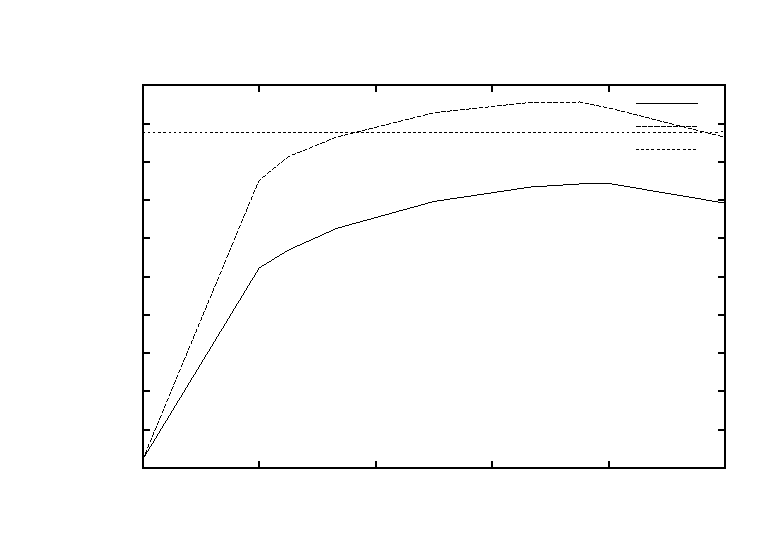
\includegraphics{chapters/chapter6/graphs/gold_division}}%
    \gplfronttext
  \end{picture}%
\endgroup
}
\caption{Prioritized items over time over specialization ratio $\tau$ for each algorithm }
\label{divisiongoldplot}
\end{figure}

\begin{figure}[!htb]
\centering
\resizebox{\textwidth}{!}{% GNUPLOT: LaTeX picture with Postscript
\begingroup
  \makeatletter
  \providecommand\color[2][]{%
    \GenericError{(gnuplot) \space\space\space\@spaces}{%
      Package color not loaded in conjunction with
      terminal option `colourtext'%
    }{See the gnuplot documentation for explanation.%
    }{Either use 'blacktext' in gnuplot or load the package
      color.sty in LaTeX.}%
    \renewcommand\color[2][]{}%
  }%
  \providecommand\includegraphics[2][]{%
    \GenericError{(gnuplot) \space\space\space\@spaces}{%
      Package graphicx or graphics not loaded%
    }{See the gnuplot documentation for explanation.%
    }{The gnuplot epslatex terminal needs graphicx.sty or graphics.sty.}%
    \renewcommand\includegraphics[2][]{}%
  }%
  \providecommand\rotatebox[2]{#2}%
  \@ifundefined{ifGPcolor}{%
    \newif\ifGPcolor
    \GPcolorfalse
  }{}%
  \@ifundefined{ifGPblacktext}{%
    \newif\ifGPblacktext
    \GPblacktexttrue
  }{}%
  % define a \g@addto@macro without @ in the name:
  \let\gplgaddtomacro\g@addto@macro
  % define empty templates for all commands taking text:
  \gdef\gplbacktext{}%
  \gdef\gplfronttext{}%
  \makeatother
  \ifGPblacktext
    % no textcolor at all
    \def\colorrgb#1{}%
    \def\colorgray#1{}%
  \else
    % gray or color?
    \ifGPcolor
      \def\colorrgb#1{\color[rgb]{#1}}%
      \def\colorgray#1{\color[gray]{#1}}%
      \expandafter\def\csname LTw\endcsname{\color{white}}%
      \expandafter\def\csname LTb\endcsname{\color{black}}%
      \expandafter\def\csname LTa\endcsname{\color{black}}%
      \expandafter\def\csname LT0\endcsname{\color[rgb]{1,0,0}}%
      \expandafter\def\csname LT1\endcsname{\color[rgb]{0,1,0}}%
      \expandafter\def\csname LT2\endcsname{\color[rgb]{0,0,1}}%
      \expandafter\def\csname LT3\endcsname{\color[rgb]{1,0,1}}%
      \expandafter\def\csname LT4\endcsname{\color[rgb]{0,1,1}}%
      \expandafter\def\csname LT5\endcsname{\color[rgb]{1,1,0}}%
      \expandafter\def\csname LT6\endcsname{\color[rgb]{0,0,0}}%
      \expandafter\def\csname LT7\endcsname{\color[rgb]{1,0.3,0}}%
      \expandafter\def\csname LT8\endcsname{\color[rgb]{0.5,0.5,0.5}}%
    \else
      % gray
      \def\colorrgb#1{\color{black}}%
      \def\colorgray#1{\color[gray]{#1}}%
      \expandafter\def\csname LTw\endcsname{\color{white}}%
      \expandafter\def\csname LTb\endcsname{\color{black}}%
      \expandafter\def\csname LTa\endcsname{\color{black}}%
      \expandafter\def\csname LT0\endcsname{\color{black}}%
      \expandafter\def\csname LT1\endcsname{\color{black}}%
      \expandafter\def\csname LT2\endcsname{\color{black}}%
      \expandafter\def\csname LT3\endcsname{\color{black}}%
      \expandafter\def\csname LT4\endcsname{\color{black}}%
      \expandafter\def\csname LT5\endcsname{\color{black}}%
      \expandafter\def\csname LT6\endcsname{\color{black}}%
      \expandafter\def\csname LT7\endcsname{\color{black}}%
      \expandafter\def\csname LT8\endcsname{\color{black}}%
    \fi
  \fi
  \setlength{\unitlength}{0.0500bp}%
  \begin{picture}(7200.00,5040.00)%
    \gplgaddtomacro\gplbacktext{%
      \csname LTb\endcsname%
      \put(1078,704){\makebox(0,0)[r]{\strut{} 0.1}}%
      \put(1078,1072){\makebox(0,0)[r]{\strut{} 0.15}}%
      \put(1078,1439){\makebox(0,0)[r]{\strut{} 0.2}}%
      \put(1078,1806){\makebox(0,0)[r]{\strut{} 0.25}}%
      \put(1078,2174){\makebox(0,0)[r]{\strut{} 0.3}}%
      \put(1078,2541){\makebox(0,0)[r]{\strut{} 0.35}}%
      \put(1078,2909){\makebox(0,0)[r]{\strut{} 0.4}}%
      \put(1078,3276){\makebox(0,0)[r]{\strut{} 0.45}}%
      \put(1078,3644){\makebox(0,0)[r]{\strut{} 0.5}}%
      \put(1078,4011){\makebox(0,0)[r]{\strut{} 0.55}}%
      \put(1078,4379){\makebox(0,0)[r]{\strut{} 0.6}}%
      \put(1210,484){\makebox(0,0){\strut{} 0}}%
      \put(2329,484){\makebox(0,0){\strut{} 0.2}}%
      \put(3447,484){\makebox(0,0){\strut{} 0.4}}%
      \put(4566,484){\makebox(0,0){\strut{} 0.6}}%
      \put(5684,484){\makebox(0,0){\strut{} 0.8}}%
      \put(6803,484){\makebox(0,0){\strut{} 1}}%
      \put(176,2541){\rotatebox{-270}{\makebox(0,0){\strut{}Non-prioritized items over time ($\tau$)}}}%
      \put(4006,154){\makebox(0,0){\strut{}Robot Specialization Ratio($\tau$)}}%
      \put(4006,4709){\makebox(0,0){\strut{}Non-prioritized items over time for each algorithm for robot specialization ratios}}%
    }%
    \gplgaddtomacro\gplfronttext{%
      \csname LTb\endcsname%
      \put(5816,4206){\makebox(0,0)[r]{\strut{}Na\"ive}}%
      \csname LTb\endcsname%
      \put(5816,3986){\makebox(0,0)[r]{\strut{}Desert Ant}}%
      \csname LTb\endcsname%
      \put(5816,3766){\makebox(0,0)[r]{\strut{}Honey Bee}}%
    }%
    \gplbacktext
    \put(0,0){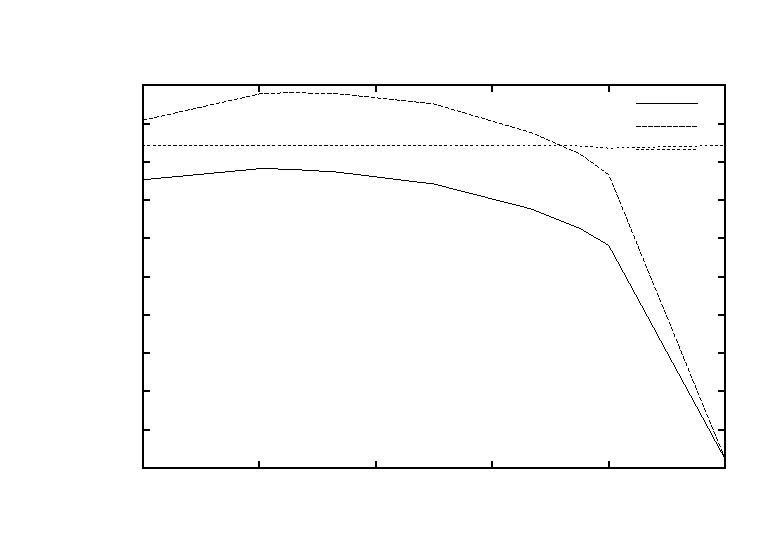
\includegraphics{chapters/chapter6/graphs/waste_division}}%
    \gplfronttext
  \end{picture}%
\endgroup
}
\caption{Non-prioritized items over time over specialization ratio $\tau$ for each algorithm}
\label{divisionwasteplot}
\end{figure}

An examination of Figure~\ref{divisiongoldplot} and Figure~\ref{divisionwasteplot} reveals some surprising observations.
As was discussed in Section~\ref{results:flexibility}, the overall trend is that as the ratio of robots foraging the prioritized type increases, the performance of the na\"ive algorithm increases. An interesting observation is that a robot specialization ratio $r=0.8$ results in the best performance for the na\"ive foraging aglorithms, while $r=1$, where all robots are foraging prioritized items, has slightly less effective performance. This can be attributed to the fact that foraging a portion of non-prioritized items benefits the algorithm.

%Discuss Desert Ant
The desert ant algorithm shows similar trends to the na\"ive algorithm with performance peaking around $r=0.8$ while the honey bee algorithm is consistent over specialization, indicating that the honey bee algorithm does indeed perform division of labour to some level of adequacy. The desert ant does however outperform the honey bee algorithm on most of the configurations. There is space for the honey bee algorithm to be optimized so to more adequately compare the algorithms, one would have to optimize the parameters. 
The performance of desert ant algorithm is interesting since there exists a configuration for $r$, $r=0.8$ that results in the best performance, independent of all environment types. That performance is better than the honey bee performance which means that a swarm of robots running the desert ant algorithm with the correct specialization ratio of robots will perform better than a honey bee algorithm at any robot specialization. 

The desert ant algorithm, however, is less robust since if an event causes a change in robot specialization ratio (for example robots becoming damaged in a rock fall), the performance of the desert ant algorithm will be affected by the change in ratio, where as the honey bee algorithm performance would remain constant due to the division of labour and it's attempts to optimize (albeit sub-optimally) the specialization ratio of robots. 

The result does make one wonder why none of the other graphs reflect the fact that the honey bee algorithm is outperformed by the desert ant algorithm. The other results and graphs in this study are most likely skewed by the experiments when $r=0$ where no desert ant robots can forage prioritized items and thus when examining results aggregated over a different parameter, the results are skewed. One should note that since the study is not focused on a comparison of performance of the various foraging algorithms, but rather an exploration in parameter sensitivity, the relative performance of the algorithms to each other is not important, however it is still an interesting result considering that since the honey bee agents can share information as well as divide their labour appropriately. 
 
Some possible reasons why the desert ant algorithm may outperform the honey bee algorithm are that:
\begin{enumerate}
	\item The honey bee division of labour does not perfectly divide labour between the item types.
	\item Honey bee algorithm has a limiting factor such as one of the unoptimized parameters $f_{max}$ and $t_{max}$. 
	\item The process of the division of labour is slowing down the algorithm to some degree.
\end{enumerate}

In terms of robustness, despite the desert ant outperforming the honey bee algorithm on certain configurations, the fact that performance of the desert ant algorithm is dependant on the initial specialization ratio of the swarm indicates that the desert ant algorithm is less robust since if large portion of robots are damaged, and the specialization ratio is thus changed, the algorithms performance may decrease significantly. The honey bee algorithm can adjust the specialization ratio of the swarm to a near optimal configuration and thus if damange to the robots causes a change in specialization ratio, the algorithm should have the ability to adapt the specialization ratio in order to maintain a gracefully degraded performance. The performance of na\"ive algorithm, similarly to the performance of desert ant algorithm is also dependant on the initial specializtion ratio as can be seen in Figure~\ref{divisiongoldplot} and Figure~\ref{divisionwasteplot}. 

\section{Scalability}
\label{results:scability}
Scalability is a key feature of swarm robotics. In order to examine the scalability of the proposed foraging algorithms, the performance of algorithms is compared over differing robot densities. 

\subsection{Robot Density}
\label{results:numberenvironments}

%Mann Whitney U tables? Needed? Yes

\begin{figure}[!htb]
\centering
\resizebox{\textwidth}{!}{% GNUPLOT: LaTeX picture with Postscript
\begingroup
  \makeatletter
  \providecommand\color[2][]{%
    \GenericError{(gnuplot) \space\space\space\@spaces}{%
      Package color not loaded in conjunction with
      terminal option `colourtext'%
    }{See the gnuplot documentation for explanation.%
    }{Either use 'blacktext' in gnuplot or load the package
      color.sty in LaTeX.}%
    \renewcommand\color[2][]{}%
  }%
  \providecommand\includegraphics[2][]{%
    \GenericError{(gnuplot) \space\space\space\@spaces}{%
      Package graphicx or graphics not loaded%
    }{See the gnuplot documentation for explanation.%
    }{The gnuplot epslatex terminal needs graphicx.sty or graphics.sty.}%
    \renewcommand\includegraphics[2][]{}%
  }%
  \providecommand\rotatebox[2]{#2}%
  \@ifundefined{ifGPcolor}{%
    \newif\ifGPcolor
    \GPcolorfalse
  }{}%
  \@ifundefined{ifGPblacktext}{%
    \newif\ifGPblacktext
    \GPblacktexttrue
  }{}%
  % define a \g@addto@macro without @ in the name:
  \let\gplgaddtomacro\g@addto@macro
  % define empty templates for all commands taking text:
  \gdef\gplbacktext{}%
  \gdef\gplfronttext{}%
  \makeatother
  \ifGPblacktext
    % no textcolor at all
    \def\colorrgb#1{}%
    \def\colorgray#1{}%
  \else
    % gray or color?
    \ifGPcolor
      \def\colorrgb#1{\color[rgb]{#1}}%
      \def\colorgray#1{\color[gray]{#1}}%
      \expandafter\def\csname LTw\endcsname{\color{white}}%
      \expandafter\def\csname LTb\endcsname{\color{black}}%
      \expandafter\def\csname LTa\endcsname{\color{black}}%
      \expandafter\def\csname LT0\endcsname{\color[rgb]{1,0,0}}%
      \expandafter\def\csname LT1\endcsname{\color[rgb]{0,1,0}}%
      \expandafter\def\csname LT2\endcsname{\color[rgb]{0,0,1}}%
      \expandafter\def\csname LT3\endcsname{\color[rgb]{1,0,1}}%
      \expandafter\def\csname LT4\endcsname{\color[rgb]{0,1,1}}%
      \expandafter\def\csname LT5\endcsname{\color[rgb]{1,1,0}}%
      \expandafter\def\csname LT6\endcsname{\color[rgb]{0,0,0}}%
      \expandafter\def\csname LT7\endcsname{\color[rgb]{1,0.3,0}}%
      \expandafter\def\csname LT8\endcsname{\color[rgb]{0.5,0.5,0.5}}%
    \else
      % gray
      \def\colorrgb#1{\color{black}}%
      \def\colorgray#1{\color[gray]{#1}}%
      \expandafter\def\csname LTw\endcsname{\color{white}}%
      \expandafter\def\csname LTb\endcsname{\color{black}}%
      \expandafter\def\csname LTa\endcsname{\color{black}}%
      \expandafter\def\csname LT0\endcsname{\color{black}}%
      \expandafter\def\csname LT1\endcsname{\color{black}}%
      \expandafter\def\csname LT2\endcsname{\color{black}}%
      \expandafter\def\csname LT3\endcsname{\color{black}}%
      \expandafter\def\csname LT4\endcsname{\color{black}}%
      \expandafter\def\csname LT5\endcsname{\color{black}}%
      \expandafter\def\csname LT6\endcsname{\color{black}}%
      \expandafter\def\csname LT7\endcsname{\color{black}}%
      \expandafter\def\csname LT8\endcsname{\color{black}}%
    \fi
  \fi
  \setlength{\unitlength}{0.0500bp}%
  \begin{picture}(7200.00,5040.00)%
    \gplgaddtomacro\gplbacktext{%
      \csname LTb\endcsname%
      \put(1078,704){\makebox(0,0)[r]{\strut{} 0.25}}%
      \put(1078,1163){\makebox(0,0)[r]{\strut{} 0.3}}%
      \put(1078,1623){\makebox(0,0)[r]{\strut{} 0.35}}%
      \put(1078,2082){\makebox(0,0)[r]{\strut{} 0.4}}%
      \put(1078,2541){\makebox(0,0)[r]{\strut{} 0.45}}%
      \put(1078,3001){\makebox(0,0)[r]{\strut{} 0.5}}%
      \put(1078,3460){\makebox(0,0)[r]{\strut{} 0.55}}%
      \put(1078,3920){\makebox(0,0)[r]{\strut{} 0.6}}%
      \put(1078,4379){\makebox(0,0)[r]{\strut{} 0.65}}%
      \put(1210,484){\makebox(0,0){\strut{} 0.1}}%
      \put(1831,484){\makebox(0,0){\strut{} 0.2}}%
      \put(2453,484){\makebox(0,0){\strut{} 0.3}}%
      \put(3074,484){\makebox(0,0){\strut{} 0.4}}%
      \put(3696,484){\makebox(0,0){\strut{} 0.5}}%
      \put(4317,484){\makebox(0,0){\strut{} 0.6}}%
      \put(4939,484){\makebox(0,0){\strut{} 0.7}}%
      \put(5560,484){\makebox(0,0){\strut{} 0.8}}%
      \put(6182,484){\makebox(0,0){\strut{} 0.9}}%
      \put(6803,484){\makebox(0,0){\strut{} 1.0}}%
      \put(176,2541){\rotatebox{-270}{\makebox(0,0){\strut{}Prioritized items over time ($\sigma$)}}}%
      \put(4006,154){\makebox(0,0){\strut{}Swarm Density($c$)}}%
      \put(4006,4709){\makebox(0,0){\strut{}Prioritized items over time for each algorithm over swarm density}}%
    }%
    \gplgaddtomacro\gplfronttext{%
      \csname LTb\endcsname%
      \put(5816,4206){\makebox(0,0)[r]{\strut{}Na\"ive}}%
      \csname LTb\endcsname%
      \put(5816,3986){\makebox(0,0)[r]{\strut{}Desert Ant}}%
      \csname LTb\endcsname%
      \put(5816,3766){\makebox(0,0)[r]{\strut{}Honey Bee}}%
    }%
    \gplbacktext
    \put(0,0){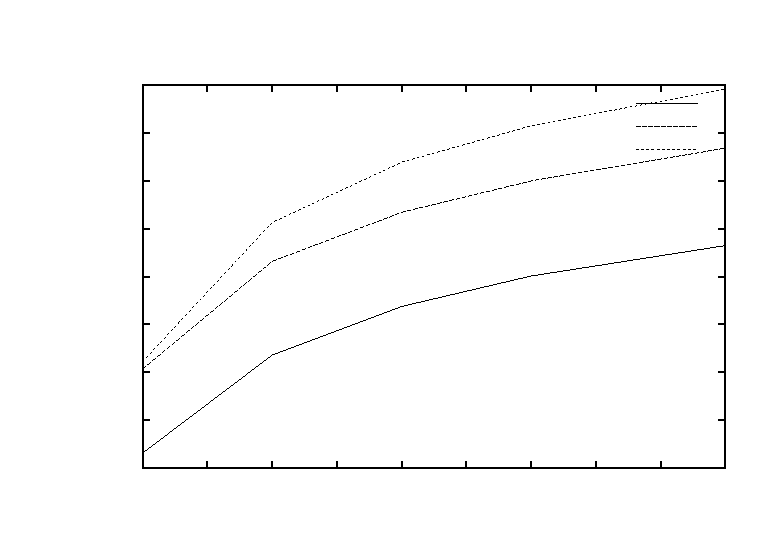
\includegraphics{chapters/chapter6/graphs/gold_robots}}%
    \gplfronttext
  \end{picture}%
\endgroup
}
\caption{Prioritized items over time over Robot Density($c$)}
\label{robotsgoldplot}
\end{figure}

\begin{figure}[!htb]
\centering
\resizebox{\textwidth}{!}{% GNUPLOT: LaTeX picture with Postscript
\begingroup
  \makeatletter
  \providecommand\color[2][]{%
    \GenericError{(gnuplot) \space\space\space\@spaces}{%
      Package color not loaded in conjunction with
      terminal option `colourtext'%
    }{See the gnuplot documentation for explanation.%
    }{Either use 'blacktext' in gnuplot or load the package
      color.sty in LaTeX.}%
    \renewcommand\color[2][]{}%
  }%
  \providecommand\includegraphics[2][]{%
    \GenericError{(gnuplot) \space\space\space\@spaces}{%
      Package graphicx or graphics not loaded%
    }{See the gnuplot documentation for explanation.%
    }{The gnuplot epslatex terminal needs graphicx.sty or graphics.sty.}%
    \renewcommand\includegraphics[2][]{}%
  }%
  \providecommand\rotatebox[2]{#2}%
  \@ifundefined{ifGPcolor}{%
    \newif\ifGPcolor
    \GPcolorfalse
  }{}%
  \@ifundefined{ifGPblacktext}{%
    \newif\ifGPblacktext
    \GPblacktexttrue
  }{}%
  % define a \g@addto@macro without @ in the name:
  \let\gplgaddtomacro\g@addto@macro
  % define empty templates for all commands taking text:
  \gdef\gplbacktext{}%
  \gdef\gplfronttext{}%
  \makeatother
  \ifGPblacktext
    % no textcolor at all
    \def\colorrgb#1{}%
    \def\colorgray#1{}%
  \else
    % gray or color?
    \ifGPcolor
      \def\colorrgb#1{\color[rgb]{#1}}%
      \def\colorgray#1{\color[gray]{#1}}%
      \expandafter\def\csname LTw\endcsname{\color{white}}%
      \expandafter\def\csname LTb\endcsname{\color{black}}%
      \expandafter\def\csname LTa\endcsname{\color{black}}%
      \expandafter\def\csname LT0\endcsname{\color[rgb]{1,0,0}}%
      \expandafter\def\csname LT1\endcsname{\color[rgb]{0,1,0}}%
      \expandafter\def\csname LT2\endcsname{\color[rgb]{0,0,1}}%
      \expandafter\def\csname LT3\endcsname{\color[rgb]{1,0,1}}%
      \expandafter\def\csname LT4\endcsname{\color[rgb]{0,1,1}}%
      \expandafter\def\csname LT5\endcsname{\color[rgb]{1,1,0}}%
      \expandafter\def\csname LT6\endcsname{\color[rgb]{0,0,0}}%
      \expandafter\def\csname LT7\endcsname{\color[rgb]{1,0.3,0}}%
      \expandafter\def\csname LT8\endcsname{\color[rgb]{0.5,0.5,0.5}}%
    \else
      % gray
      \def\colorrgb#1{\color{black}}%
      \def\colorgray#1{\color[gray]{#1}}%
      \expandafter\def\csname LTw\endcsname{\color{white}}%
      \expandafter\def\csname LTb\endcsname{\color{black}}%
      \expandafter\def\csname LTa\endcsname{\color{black}}%
      \expandafter\def\csname LT0\endcsname{\color{black}}%
      \expandafter\def\csname LT1\endcsname{\color{black}}%
      \expandafter\def\csname LT2\endcsname{\color{black}}%
      \expandafter\def\csname LT3\endcsname{\color{black}}%
      \expandafter\def\csname LT4\endcsname{\color{black}}%
      \expandafter\def\csname LT5\endcsname{\color{black}}%
      \expandafter\def\csname LT6\endcsname{\color{black}}%
      \expandafter\def\csname LT7\endcsname{\color{black}}%
      \expandafter\def\csname LT8\endcsname{\color{black}}%
    \fi
  \fi
  \setlength{\unitlength}{0.0500bp}%
  \begin{picture}(7200.00,5040.00)%
    \gplgaddtomacro\gplbacktext{%
      \csname LTb\endcsname%
      \put(1078,704){\makebox(0,0)[r]{\strut{} 0.25}}%
      \put(1078,1071){\makebox(0,0)[r]{\strut{} 0.3}}%
      \put(1078,1439){\makebox(0,0)[r]{\strut{} 0.35}}%
      \put(1078,1806){\makebox(0,0)[r]{\strut{} 0.4}}%
      \put(1078,2174){\makebox(0,0)[r]{\strut{} 0.45}}%
      \put(1078,2541){\makebox(0,0)[r]{\strut{} 0.5}}%
      \put(1078,2909){\makebox(0,0)[r]{\strut{} 0.55}}%
      \put(1078,3276){\makebox(0,0)[r]{\strut{} 0.6}}%
      \put(1078,3644){\makebox(0,0)[r]{\strut{} 0.65}}%
      \put(1078,4012){\makebox(0,0)[r]{\strut{} 0.7}}%
      \put(1078,4379){\makebox(0,0)[r]{\strut{} 0.75}}%
      \put(1210,484){\makebox(0,0){\strut{} 0}}%
      \put(1831,484){\makebox(0,0){\strut{} 10}}%
      \put(2453,484){\makebox(0,0){\strut{} 20}}%
      \put(3074,484){\makebox(0,0){\strut{} 30}}%
      \put(3696,484){\makebox(0,0){\strut{} 40}}%
      \put(4317,484){\makebox(0,0){\strut{} 50}}%
      \put(4939,484){\makebox(0,0){\strut{} 60}}%
      \put(5560,484){\makebox(0,0){\strut{} 70}}%
      \put(6182,484){\makebox(0,0){\strut{} 80}}%
      \put(6803,484){\makebox(0,0){\strut{} 90}}%
      \put(176,2541){\rotatebox{-270}{\makebox(0,0){\strut{}Non-prioritized items over time ($\sigma$)}}}%
      \put(4006,154){\makebox(0,0){\strut{}Quantity of Robots ($c$)}}%
      \put(4006,4709){\makebox(0,0){\strut{}Non-prioritized items over time for each algorithm over robot percentages}}%
    }%
    \gplgaddtomacro\gplfronttext{%
      \csname LTb\endcsname%
      \put(5816,4206){\makebox(0,0)[r]{\strut{}Na\"ive}}%
      \csname LTb\endcsname%
      \put(5816,3986){\makebox(0,0)[r]{\strut{}Desert Ant}}%
      \csname LTb\endcsname%
      \put(5816,3766){\makebox(0,0)[r]{\strut{}Honey Bee}}%
    }%
    \gplbacktext
    \put(0,0){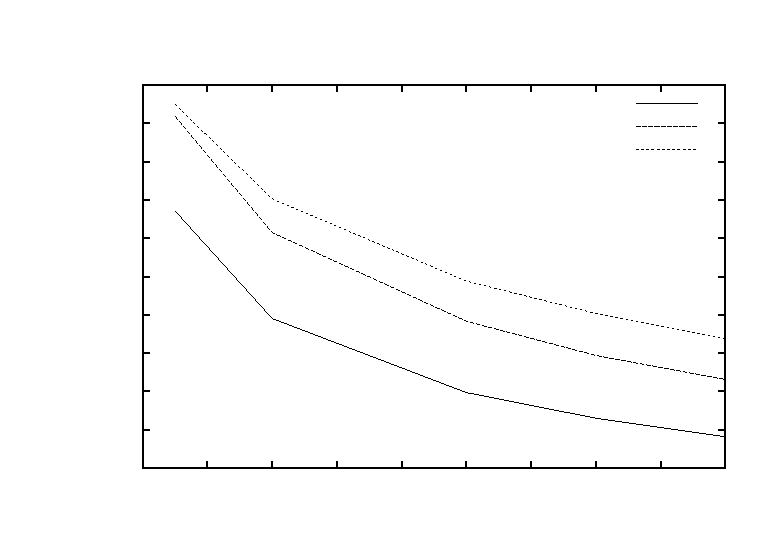
\includegraphics{chapters/chapter6/graphs/waste_robots}}%
    \gplfronttext
  \end{picture}%
\endgroup
}
\caption{Non-prioritized items over time over Robot Density ($c$)}
\label{robotswasteplot}
\end{figure}

%Discussion
The purpose of examining the effect of additional robots is to determine whether the addition of extra robots negatively effects an algorithm's performance. An algorithm that would scale perfectly would show a linear increase in performance as the number of robots increases. The addition of more robots could potentially create interference between the robots or cause malfunction of the algorithms and impacting scalability. 

A slow down of the rate of increase as the robot density ($c$) increases could also mean that the robots are just successfully foraging the entire environment with a lesser robot density which will explain as the number of robots increases, the performance does not increase. In order to avoid the situation where the entire environment is foraged, analysis should only be performed on large, high density environments where $S >= 200$ and $p >= 0.8$

The hypothesis is that the honey bee algorithm would be the least impacted by the increase in robot density since the robots will rest if they have not foraged an item for a particular period and thus the an increase in robots would not cause as much of an increase in interference. One needs to take care when selecting the environments for analysis. In order to confirm that any analysis about the slow down in the rate of foraging is caused by the increase in robot density, one should only analyse environments where the robots are unable to complete foraging of all items for all robot densities. For this reason, the analysis has only been performed over a high object density where all items were not able to be foraged at any given robot density.

%TODO: Get graph and do analysis
\subsection{Energy}
\label{results:energy}

%GET THIS GRAPH
Since energy usage was not the focus of this study, the process of assigning and monitoring energy usage to the various foraging tasks was not performed and was not considered a major metric for this study. However it is worth mentioning that the honey bee algorithm does have some waiting time where less or no energy would be spent, where as the na\"ive and desert ant algorithms do not save energy by going into a hibernation or resting state. It is thus potentially worth analysing the amount of time that the robots spend waiting at the sink in the honey bee algorithm to see if energy saving actually occurred due to active to inactive forager division of labour capabilities of the honey bee algorithm. 

One would expect the amount of time spent waiting to increase as robot density increases and the environment becomes saturated by robots since more robots would fail to find items and return to the waiting state. The graph indicates that a surprisingly small amount of time was spent waiting at the sink regardless of the robot density which tends to imply that there is room for improvement in the active to inactive forager division of labour strategy such that robots are more inefficient robots. 

One should also keep in mind that although this seems to imply that the honey bee algorithm performs more efficiently, the comparison is quite limited since the task of direct communication is likely to, in practice, be a very expensive activity energy-wise.

\subsection{Environment Size}
\label{results:environmentsize}

%As environment size increases, how does the algorithm performance suffer

%Mann whitney U + average etc etc
%Graphs compareing performacne of # robots, per algorith, for each performance measure 2 performance measures

%NEED TABLES!!!!!!!!!

\begin{figure}[!htb]
\centering
\resizebox{\textwidth}{!}{% GNUPLOT: LaTeX picture with Postscript
\begingroup
  \makeatletter
  \providecommand\color[2][]{%
    \GenericError{(gnuplot) \space\space\space\@spaces}{%
      Package color not loaded in conjunction with
      terminal option `colourtext'%
    }{See the gnuplot documentation for explanation.%
    }{Either use 'blacktext' in gnuplot or load the package
      color.sty in LaTeX.}%
    \renewcommand\color[2][]{}%
  }%
  \providecommand\includegraphics[2][]{%
    \GenericError{(gnuplot) \space\space\space\@spaces}{%
      Package graphicx or graphics not loaded%
    }{See the gnuplot documentation for explanation.%
    }{The gnuplot epslatex terminal needs graphicx.sty or graphics.sty.}%
    \renewcommand\includegraphics[2][]{}%
  }%
  \providecommand\rotatebox[2]{#2}%
  \@ifundefined{ifGPcolor}{%
    \newif\ifGPcolor
    \GPcolorfalse
  }{}%
  \@ifundefined{ifGPblacktext}{%
    \newif\ifGPblacktext
    \GPblacktexttrue
  }{}%
  % define a \g@addto@macro without @ in the name:
  \let\gplgaddtomacro\g@addto@macro
  % define empty templates for all commands taking text:
  \gdef\gplbacktext{}%
  \gdef\gplfronttext{}%
  \makeatother
  \ifGPblacktext
    % no textcolor at all
    \def\colorrgb#1{}%
    \def\colorgray#1{}%
  \else
    % gray or color?
    \ifGPcolor
      \def\colorrgb#1{\color[rgb]{#1}}%
      \def\colorgray#1{\color[gray]{#1}}%
      \expandafter\def\csname LTw\endcsname{\color{white}}%
      \expandafter\def\csname LTb\endcsname{\color{black}}%
      \expandafter\def\csname LTa\endcsname{\color{black}}%
      \expandafter\def\csname LT0\endcsname{\color[rgb]{1,0,0}}%
      \expandafter\def\csname LT1\endcsname{\color[rgb]{0,1,0}}%
      \expandafter\def\csname LT2\endcsname{\color[rgb]{0,0,1}}%
      \expandafter\def\csname LT3\endcsname{\color[rgb]{1,0,1}}%
      \expandafter\def\csname LT4\endcsname{\color[rgb]{0,1,1}}%
      \expandafter\def\csname LT5\endcsname{\color[rgb]{1,1,0}}%
      \expandafter\def\csname LT6\endcsname{\color[rgb]{0,0,0}}%
      \expandafter\def\csname LT7\endcsname{\color[rgb]{1,0.3,0}}%
      \expandafter\def\csname LT8\endcsname{\color[rgb]{0.5,0.5,0.5}}%
    \else
      % gray
      \def\colorrgb#1{\color{black}}%
      \def\colorgray#1{\color[gray]{#1}}%
      \expandafter\def\csname LTw\endcsname{\color{white}}%
      \expandafter\def\csname LTb\endcsname{\color{black}}%
      \expandafter\def\csname LTa\endcsname{\color{black}}%
      \expandafter\def\csname LT0\endcsname{\color{black}}%
      \expandafter\def\csname LT1\endcsname{\color{black}}%
      \expandafter\def\csname LT2\endcsname{\color{black}}%
      \expandafter\def\csname LT3\endcsname{\color{black}}%
      \expandafter\def\csname LT4\endcsname{\color{black}}%
      \expandafter\def\csname LT5\endcsname{\color{black}}%
      \expandafter\def\csname LT6\endcsname{\color{black}}%
      \expandafter\def\csname LT7\endcsname{\color{black}}%
      \expandafter\def\csname LT8\endcsname{\color{black}}%
    \fi
  \fi
  \setlength{\unitlength}{0.0500bp}%
  \begin{picture}(7200.00,5040.00)%
    \gplgaddtomacro\gplbacktext{%
      \csname LTb\endcsname%
      \put(946,704){\makebox(0,0)[r]{\strut{} 0.1}}%
      \put(946,1112){\makebox(0,0)[r]{\strut{} 0.2}}%
      \put(946,1521){\makebox(0,0)[r]{\strut{} 0.3}}%
      \put(946,1929){\makebox(0,0)[r]{\strut{} 0.4}}%
      \put(946,2337){\makebox(0,0)[r]{\strut{} 0.5}}%
      \put(946,2746){\makebox(0,0)[r]{\strut{} 0.6}}%
      \put(946,3154){\makebox(0,0)[r]{\strut{} 0.7}}%
      \put(946,3562){\makebox(0,0)[r]{\strut{} 0.8}}%
      \put(946,3971){\makebox(0,0)[r]{\strut{} 0.9}}%
      \put(946,4379){\makebox(0,0)[r]{\strut{} 1}}%
      \put(1078,484){\makebox(0,0){\strut{} 50}}%
      \put(1714,484){\makebox(0,0){\strut{} 100}}%
      \put(2350,484){\makebox(0,0){\strut{} 150}}%
      \put(2986,484){\makebox(0,0){\strut{} 200}}%
      \put(3622,484){\makebox(0,0){\strut{} 250}}%
      \put(4259,484){\makebox(0,0){\strut{} 300}}%
      \put(4895,484){\makebox(0,0){\strut{} 350}}%
      \put(5531,484){\makebox(0,0){\strut{} 400}}%
      \put(6167,484){\makebox(0,0){\strut{} 450}}%
      \put(6803,484){\makebox(0,0){\strut{} 500}}%
      \put(176,2541){\rotatebox{-270}{\makebox(0,0){\strut{}Prioritized items over time ($\sigma$)}}}%
      \put(3940,154){\makebox(0,0){\strut{}Size ($S$)}}%
      \put(3940,4709){\makebox(0,0){\strut{}Prioritized items over time for each algorithm for different grid sizes}}%
    }%
    \gplgaddtomacro\gplfronttext{%
      \csname LTb\endcsname%
      \put(5816,4206){\makebox(0,0)[r]{\strut{}Na\"ive}}%
      \csname LTb\endcsname%
      \put(5816,3986){\makebox(0,0)[r]{\strut{}Desert Ant}}%
      \csname LTb\endcsname%
      \put(5816,3766){\makebox(0,0)[r]{\strut{}Honey Bee}}%
    }%
    \gplbacktext
    \put(0,0){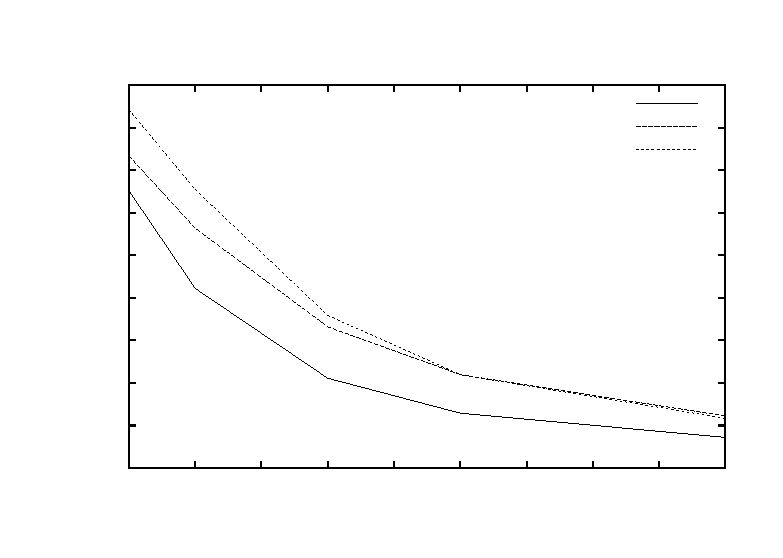
\includegraphics{chapters/chapter6/graphs/gold_sizes}}%
    \gplfronttext
  \end{picture}%
\endgroup
}
\caption{Environment Size}
\label{sizegoldplot}
\end{figure}

\begin{figure}[!htb]
\centering
\resizebox{\textwidth}{!}{% GNUPLOT: LaTeX picture with Postscript
\begingroup
  \makeatletter
  \providecommand\color[2][]{%
    \GenericError{(gnuplot) \space\space\space\@spaces}{%
      Package color not loaded in conjunction with
      terminal option `colourtext'%
    }{See the gnuplot documentation for explanation.%
    }{Either use 'blacktext' in gnuplot or load the package
      color.sty in LaTeX.}%
    \renewcommand\color[2][]{}%
  }%
  \providecommand\includegraphics[2][]{%
    \GenericError{(gnuplot) \space\space\space\@spaces}{%
      Package graphicx or graphics not loaded%
    }{See the gnuplot documentation for explanation.%
    }{The gnuplot epslatex terminal needs graphicx.sty or graphics.sty.}%
    \renewcommand\includegraphics[2][]{}%
  }%
  \providecommand\rotatebox[2]{#2}%
  \@ifundefined{ifGPcolor}{%
    \newif\ifGPcolor
    \GPcolorfalse
  }{}%
  \@ifundefined{ifGPblacktext}{%
    \newif\ifGPblacktext
    \GPblacktexttrue
  }{}%
  % define a \g@addto@macro without @ in the name:
  \let\gplgaddtomacro\g@addto@macro
  % define empty templates for all commands taking text:
  \gdef\gplbacktext{}%
  \gdef\gplfronttext{}%
  \makeatother
  \ifGPblacktext
    % no textcolor at all
    \def\colorrgb#1{}%
    \def\colorgray#1{}%
  \else
    % gray or color?
    \ifGPcolor
      \def\colorrgb#1{\color[rgb]{#1}}%
      \def\colorgray#1{\color[gray]{#1}}%
      \expandafter\def\csname LTw\endcsname{\color{white}}%
      \expandafter\def\csname LTb\endcsname{\color{black}}%
      \expandafter\def\csname LTa\endcsname{\color{black}}%
      \expandafter\def\csname LT0\endcsname{\color[rgb]{1,0,0}}%
      \expandafter\def\csname LT1\endcsname{\color[rgb]{0,1,0}}%
      \expandafter\def\csname LT2\endcsname{\color[rgb]{0,0,1}}%
      \expandafter\def\csname LT3\endcsname{\color[rgb]{1,0,1}}%
      \expandafter\def\csname LT4\endcsname{\color[rgb]{0,1,1}}%
      \expandafter\def\csname LT5\endcsname{\color[rgb]{1,1,0}}%
      \expandafter\def\csname LT6\endcsname{\color[rgb]{0,0,0}}%
      \expandafter\def\csname LT7\endcsname{\color[rgb]{1,0.3,0}}%
      \expandafter\def\csname LT8\endcsname{\color[rgb]{0.5,0.5,0.5}}%
    \else
      % gray
      \def\colorrgb#1{\color{black}}%
      \def\colorgray#1{\color[gray]{#1}}%
      \expandafter\def\csname LTw\endcsname{\color{white}}%
      \expandafter\def\csname LTb\endcsname{\color{black}}%
      \expandafter\def\csname LTa\endcsname{\color{black}}%
      \expandafter\def\csname LT0\endcsname{\color{black}}%
      \expandafter\def\csname LT1\endcsname{\color{black}}%
      \expandafter\def\csname LT2\endcsname{\color{black}}%
      \expandafter\def\csname LT3\endcsname{\color{black}}%
      \expandafter\def\csname LT4\endcsname{\color{black}}%
      \expandafter\def\csname LT5\endcsname{\color{black}}%
      \expandafter\def\csname LT6\endcsname{\color{black}}%
      \expandafter\def\csname LT7\endcsname{\color{black}}%
      \expandafter\def\csname LT8\endcsname{\color{black}}%
    \fi
  \fi
  \setlength{\unitlength}{0.0500bp}%
  \begin{picture}(7200.00,5040.00)%
    \gplgaddtomacro\gplbacktext{%
      \csname LTb\endcsname%
      \put(946,704){\makebox(0,0)[r]{\strut{} 0.1}}%
      \put(946,1112){\makebox(0,0)[r]{\strut{} 0.2}}%
      \put(946,1521){\makebox(0,0)[r]{\strut{} 0.3}}%
      \put(946,1929){\makebox(0,0)[r]{\strut{} 0.4}}%
      \put(946,2337){\makebox(0,0)[r]{\strut{} 0.5}}%
      \put(946,2746){\makebox(0,0)[r]{\strut{} 0.6}}%
      \put(946,3154){\makebox(0,0)[r]{\strut{} 0.7}}%
      \put(946,3562){\makebox(0,0)[r]{\strut{} 0.8}}%
      \put(946,3971){\makebox(0,0)[r]{\strut{} 0.9}}%
      \put(946,4379){\makebox(0,0)[r]{\strut{} 1}}%
      \put(1078,484){\makebox(0,0){\strut{} 50}}%
      \put(1714,484){\makebox(0,0){\strut{} 100}}%
      \put(2350,484){\makebox(0,0){\strut{} 150}}%
      \put(2986,484){\makebox(0,0){\strut{} 200}}%
      \put(3622,484){\makebox(0,0){\strut{} 250}}%
      \put(4259,484){\makebox(0,0){\strut{} 300}}%
      \put(4895,484){\makebox(0,0){\strut{} 350}}%
      \put(5531,484){\makebox(0,0){\strut{} 400}}%
      \put(6167,484){\makebox(0,0){\strut{} 450}}%
      \put(6803,484){\makebox(0,0){\strut{} 500}}%
      \put(176,2541){\rotatebox{-270}{\makebox(0,0){\strut{}Non-prioritized items over time ($\sigma$)}}}%
      \put(3940,154){\makebox(0,0){\strut{}Size ($S$)}}%
      \put(3940,4709){\makebox(0,0){\strut{}Non-prioritized items over time for each algorithm for different grid sizes}}%
    }%
    \gplgaddtomacro\gplfronttext{%
      \csname LTb\endcsname%
      \put(5816,4206){\makebox(0,0)[r]{\strut{}Na\"ive}}%
      \csname LTb\endcsname%
      \put(5816,3986){\makebox(0,0)[r]{\strut{}Desert Ant}}%
      \csname LTb\endcsname%
      \put(5816,3766){\makebox(0,0)[r]{\strut{}Honey Bee}}%
    }%
    \gplbacktext
    \put(0,0){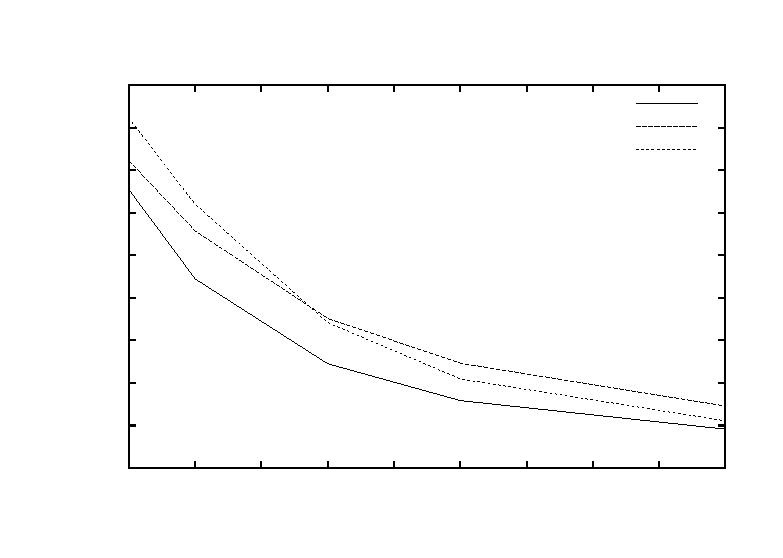
\includegraphics{chapters/chapter6/graphs/waste_sizes}}%
    \gplfronttext
  \end{picture}%
\endgroup
}
\caption{Non-prioritized items over time for different environment sizes for each algorithm}
\label{sizewasteplot}
\end{figure}

%Need help here
As the environment size increases, one would expect the performance to get quadratically less since the algorithms were run for the same amount of time. For this analysis, the experiments would ideally be run until no more items can be foraged, but due to time constraints only a limited study could be performed. For this reasons, the results have been presented however no valid analysis can be performed.

\section{Summary}
\label{results:summary}

%%%%%%%%%%%%%%%%%%%%%%%%%%%%%%%%%%%%%%%%%%%%%%%%%
%%%%%%%%%%%%%%%%%%%%%%%%%%%%%%%%%%%%%%%%%%%%%%%%%